\documentclass[a4paper,11pt,german]{report}

\usepackage[ngerman]{babel}   % deutsche Sprachanpassung
\usepackage[utf8]{inputenc} % erlaubt Umlaute in der tex-Datei
\usepackage[T1]{fontenc}      % Trennung bei Wörtern mit Umlauten
\usepackage[DIV15]{typearea}  % Vergrößerung des Textbereichs
\usepackage{amsmath}
\usepackage{amsfonts}
\usepackage{amssymb}
\usepackage{amsthm}
\usepackage{units}	
\usepackage{esvect}
\usepackage{ wasysym }
\usepackage{wrapfig}
\usepackage{graphicx} %graphiken einfügen
\usepackage{floatflt} % graphik als fließtext
\usepackage[framemethod=tikz]{mdframed} %Rahmen für Boxen
\usepackage{ulem} %Unterschtreichen 
\usepackage{enumitem}
\usepackage{float}
\usepackage{gauss}
\usepackage{tikz}
\usepackage{pgfplots}
\usepgfplotslibrary{fillbetween}

%\usepackage{tabular}
%%%%%%%%%%%%%%%%%%%% KOPF-ZEILE %%%%%%%%%%%%%%%%%%%%		

\makeatletter
\renewcommand*\env@matrix[1][*\c@MaxMatrixCols c]{%
  \hskip -\arraycolsep
  \let\@ifnextchar\new@ifnextchar
  \array{#1}}
\makeatother

\usepackage{etoolbox}
\makeatletter
\patchcmd\g@matrix
 {\vbox\bgroup}
 {\vbox\bgroup\normalbaselines}% restore the standard baselineskip
 {}{}
\makeatother


\newcommand{\BAR}{%
  \hspace{-\arraycolsep}%
  \strut\vrule % the `\vrule` is as high and deep as a strut
  \hspace{-\arraycolsep}%
}

%Kopf- und Fußzeile
\usepackage{fancyhdr}
\pagestyle{fancy}
%Kopfzeile links bzw. innen
\fancyhead[L]{\normalsize\textbf{Testklausur 2020}}
%Kopfzeile mittig
\fancyhead[C]{\normalsize\textbf{Teil I: Offene Aufgaben}}
%Kopfzeile rechts bzw. außen
\fancyhead[R]{\normalsize\textbf{Glemser Learning}}
%Linie oben
\renewcommand{\headrulewidth}{0.5pt}
\cfoot{Testklausur 2020 - \thepage}
%%%%%%%%%%%%%%%%%%%%%%%%%%%%%%%%%%%%%%%%%%%%%%%%%%%%%%%
%%%% KEIN EINRÜCKEN %%%%%%%%%%%%%%%%%%%%
\setlength{\parindent}{0cm}	
%%%%%%%%%%%%%%%%%%%%%%%%%%%%%%%%%%%%%%				




%\cfoot{Testklausur 2019 - Seite \thepage}
\setcounter{page}{1}



\newcommand{\td}[1]{\text{\rmfamily d} #1}
\newcommand{\aufgabe}[2]{(#1) (#2 Punkte)}
\newcommand{\frage}[2]{Frage #1 (#2 Punkte)}			
\allowdisplaybreaks	
%% \begin{document}	- Textanfang!	
\begin{document}


%\newcommand{\ein}[2]{(#1) (#2 Punkte)}


\begin{Large}
\textbf{Teil I: Offene Aufgaben (36 Punkte)}
\end{Large}
\\
\\
\\
\textbf{Allgemeine Anweisungen für offene Fragen:}
\\
\renewcommand{\labelenumi}{(\roman{enumi})}
\begin{enumerate}
\item
Ihre Antworten müssen alle Rechenschritte enthalten,
diese müssen klar ersichtlich sein.
Verwendung korrekter mathematischer Notation wird erwartet
und fliesst in die Bewertung ein.

\item
Ihre Antworten zu den jeweiligen Teilaufgaben müssen in den dafür vorgesehenen Platz geschrie-
ben werden. Sollte dieser Platz nicht ausreichen, setzen Sie Ihre Antwort auf der Rückseite oder
dem separat zur Verfügung gestellten Papier fort. Verweisen Sie in solchen Fällen ausdrücklich
auf Ihre Fortsetzung. Bitte schreiben Sie zudem Ihren Vor- und Nachnamen auf jeden separaten
Lösungsbogen.

\item
Es werden nur Antworten im dafür vorgesehenen Platz bewertet. Antworten auf der Rückseite
oder separatem Papier werden nur bei einem vorhandenen und klaren Verweis darauf bewertet.

\item
Die Teilaufgaben werden mit den jeweils oben auf der Seite angegebenen Punkten bewertet.

\item
Ihre endgültige Lösung jeder Teilaufgabe darf nur eine einzige Version enthalten.

\item
Zwischenrechnungen und Notizen müssen auf einem getrennten Blatt gemacht werden. Diese
Blätter müssen, deutlich als Entwurf gekennzeichnet, ebenfalls abgegeben werden.
\end{enumerate}

\newpage
\section*{\hfil Aufgaben \hfil}
\vspace{1cm}
\section*{Aufgabe 1 (36 Punkte)}
\vspace{0.4cm}
%\titleformat{\subsection}[runin]
%{\normalfont\large\bfseries}{\thesubsection}{1em}{}
\subsection*{\aufgabe{a1}{6}} 
Thomas Robert Malthus (1766-1834), ein britischer Ökonom und Pfarrer, veröffentlichte
1798 seinen vielbeachteten \textit{Essay on the Principle of Population}.
Er formulierte das Axiom, dass die Weltbevölkerung exponentiell wachse, die Nahrung dagegen nur linear. 
Das bedeutet, dass die Funktion $ n(t) $, welche die Anzahl Menschen angibt, die man bei optimaler Verteilung der zur Verfügung stehenden Nahrungsmittel zu Zeit $ t $ ernähren könnte, eine lineare ist:
\begin{align*}
	n(t) = a + b \cdot t.
\end{align*}
Die Weltbevölkerung $ w(t) $ betrug im Jahre 1800 ($ t= 0 $) rund eine Milliarde, d.h. $ w(0) = 10^9 $.
Wir wollen annehmen, dass die Weltbevölkerung rund $ 1\% $ pro Jahr wächst.
Außerdem wollen wir mit
\begin{align*}
	a = 2 \cdot 10^9 \ \textrm{und} \ b = 0.2 \cdot 10^9
\end{align*}
rechnen.
\begin{description}
	\item[Beweisen Sie:] 
	Es gibt genau einen Zeitpunkt $ t^\star > 400 $, an dem die Weltbevölkerung gerade noch ernährt werden kann, d.h., für $ w(t^\star)  = n(t^\star )$ ist.
\end{description}  
\
\\


\subsection*{\aufgabe{a2}{6}}
Thomas Robert Malthus (1766-1834), ein britischer Ökonom und Pfarrer, veröffentlichte
1798 seinen vielbeachteten \textit{Essay on the Principle of Population}.
Er formulierte das Axiom, dass die Weltbevölkerung exponentiell wachse, die Nahrung dagegen nur linear. 
Das bedeutet, dass die Funktion $ n(t) $, welche die Anzahl Menschen angibt, die man bei optimaler Verteilung der zur Verfügung stehenden Nahrungsmittel zu Zeit $ t $ ernähren könnte, eine lineare ist:
\begin{align*}
	n(t) = a + b \cdot t.
\end{align*}
Die Weltbevölkerung $ w(t) $ betrug im Jahre 1800 ($ t= 0 $) rund eine Milliarde, d.h. $ w(0) = 10^9 $.
Wir wollen annehmen, dass die Weltbevölkerung rund $ 1\% $ pro Jahr wächst.
Außerdem wollen wir mit
\begin{align*}
	a = 2 \cdot 10^9 \ \textrm{und} \ b = 0.2 \cdot 10^9
\end{align*}
rechnen.\\
\\
Es gibt genau einen Zeitpunkt $ t^\star > 400 $, an dem die Weltbevölkerung gerade noch ernährt werden kann, d.h., für $ w(t^\star)  = n(t^\star )$ ist.\\
\\
Verwenden Sie eine Taylor-Approximation zweiter Ordnung im Punkt $ t_0 = 400 $, um eine Näherung für $ t^\star $ zu finden.
 \\
\\
\titleformat{\subsection}[display]
{\normalfont\large\bfseries}{\thesubsection}{1mm}{}
\subsection*{\aufgabe{b}{10}}
Max hat über seine Verhältnisse gelebt. 
Deshalb hat er nun Schulden von mehreren hunderttausend Franken.
Die Schuldenberatung vermittelt ihm am Anfang des Jahres einen Privatkredit mit $ i = 5 \% $ in der genannten Höhe von $ S = 355'000 \ [\textrm{CHF}] $, den er in $ 12 $ gleich grossen Raten $ C $ jeweils per Jahresende abbezahlen muss. 
\begin{enumerate}
	\item[(b1)] Fügen Sie die Ereignisse und Mittelflüsse dem Zeitstrahl hinzu.
	\item[(b2)] Berechnen Sie die Höhe der Ratenzahlung $ C $.
\end{enumerate}
Am Ende des vierten Jahres gewinnt Max im Lotto CHF $ 160'000 $.
Er beschließt in diesem Jahr statt der normalen Rate $ C $ den ganzen Lottogewinn zur Abzahlung des Kredits zu benützen.
\begin{enumerate}
	\item[(b3)] Ergänzen Sie die Information am Zeitstrahl und berechnen Sie die Restschuld $ \overline{S} $ nach der Einzahlung am Ende des vierten Jahres.
\end{enumerate}
Max zahlt nun weiter am Ende jeden Jahres den Betrag $ C $ zu Tilgung seiner Restschuld $ \overline{S} $.
\begin{enumerate}
	\item[(b4)] Wie viele Zahlungen muss er machen, bis er die Restschuld vollkommen getilgt hat?
	\item[(b5)] Mit der letzten Rate muss nicht mehr der komplette Betrag $ C $ geleistet werden. Wie hoch ist die Zahlung genau?
\end{enumerate}
\begin{center}
	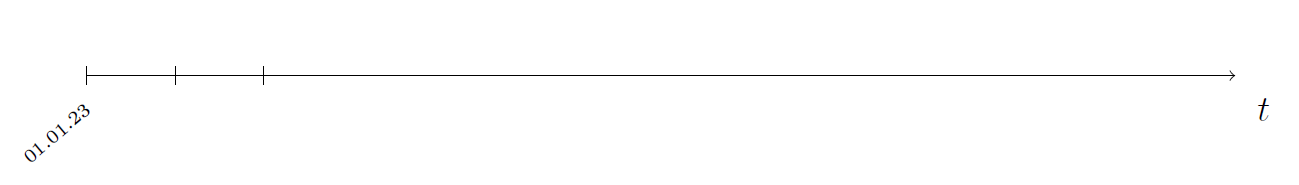
\includegraphics[scale=0.3]{pictures/zeitstrahl_1_b}
\end{center}
\ \\
\subsection*{\aufgabe{c}{6}}
Nach der Relativitätstheorie gilt für die Masse $ m $ eines Körpers, der sich mit der Geschwindigkeit $ v $ bewegt
\begin{align*}
	m(v)
	=
	\frac{m_0}{\sqrt{1 - \frac{v^2}{c^2}}}.
\end{align*}
Dabei ist $ c $ die Lichtgeschwindigkeit $ (299'792'458 \nicefrac{m}{s}) $ und $ m_0 $ die Masse in Ruhe.
\begin{enumerate}
	\item[(c1)] Berechnen Sie die Elastizität $ \varepsilon_m $ von $ m(v) $.
	\item[(c2)] Um wie viel Prozent ändert sich näherungsweise die Masse, wenn die Geschwindigkeit von $ v_0 = 0.5c $ um $ 5 \% $ erhöht wird?
\end{enumerate}
\
\\
\subsection*{\aufgabe{d}{8}}
Bei einer Absatzmenge $ x \geq 20  $ kann ein Monopolist mit dem Ertrag $ E(x) $ und den Kosten $ K(x) $ rechnen, die wie folgt gegeben sind:
\begin{align*}
	E(x) = -0.5 x^{1.5} +100 x \ \textrm{und} \ K(x) = -200\sqrt{x} + 50 x +120.
\end{align*}
Von seinem Bruttogewinn muss der Hersteller $ i \% $  $ (0 < i < 100) $ an Steuern bezahlen.
\begin{enumerate}
	\item[(d1)]
	Drücken Sie den Gewinn $ G(x) $ nach Steuern in Abhängigkeit der verkauften Menge $ x $ aus.
	\item[(d2)] 
	Für welche Menge $ x^\star $ maximiert der Hersteller seinen Gewinn nach Steuern?
\end{enumerate}


\newpage


\fancyhead[C]{\normalsize\textbf{$\qquad$ Teil II: Multiple-Choice}}
\begin{Large}
\textbf{Teil II: Multiple-Choice-Fragen (64 Punkte)}
\end{Large}
\\
\\
\\
\textbf{Allgemeine Anweisungen für Multiple-Choice-Fragen:}
\\
\renewcommand{\labelenumi}{(\roman{enumi})}
\begin{enumerate}
\item
Die Antworten auf die Multiple-Choice-Fragen müssen im dafür vorgesehenen Antwortbogen ein-
getragen werden. Es werden ausschliesslich Antworten auf diesem Antwortbogen bewertet. Der
Platz unter den Fragen ist nur für Notizen vorgesehen und wird nicht korrigiert.

\item
Jede Frage hat nur eine richtige Antwort. Es muss also auch jeweils nur eine Antwort angekreuzt werden.

\item
Falls mehrere Antworten angekreuzt sind, wird die Antwort mit 0 Punkten bewertet, auch wenn
die korrekte Antwort unter den angekreuzten ist.

\item
Bitte lesen Sie die Fragen und die Anweisungen auf dem Multiple-Choice-Antwortbogen sorgfältig.

\end{enumerate}
\newpage
\section*{Aufgabe 2 (34 Punkte)}
\vspace{0.4cm}

\subsection*{\frage{1}{3}}
$ A $ und $ B $ seien zwei Aussagen. Die zusammengesetzte Aussage
\begin{align*}
	\neg (A \ \Rightarrow \ \neg B)
\end{align*}
ist äquivalent zu 
 \renewcommand{\labelenumi}{(\alph{enumi})}
\begin{enumerate}
\item $ A \vee B $.
\item $ A \wedge B $.
\item $ (\neg A) \vee (\neg B)$
\item $ (\neg A) \wedge (\neg B)$.
\end{enumerate}
\ \\
\subsection*{\frage{2}{2}}
Die Folge $ \lbrace a_n \rbrace_{n \in \N} $ ist monoton wachsend und konvergiert mit $ \lim_{n \to \infty} a_n = -2 $.
Die Folge $ \lbrace b_n \rbrace_{n \in \N} $ ist definiert durch $ b_n = (-3) \cdot a_n $.\\
\\
Dann folgt:
\renewcommand{\labelenumi}{(\alph{enumi})}
\begin{enumerate}
\item $ \lbrace b_n \rbrace_{n \in \N} $ ist monoton wachsend und divergent.
\item $ \lbrace b_n \rbrace_{n \in \N} $ ist monoton wachsend und konvergent.
\item $ \lbrace b_n \rbrace_{n \in \N} $ ist monoton fallend und divergent.
\item $ \lbrace b_n \rbrace_{n \in \N} $ ist monoton fallend und konvergent.
\item $ \lbrace b_n \rbrace_{n \in \N} $ ist nicht monoton und divergent.
\end{enumerate}
\ \\
\subsection*{\frage{3}{3}}
Eine Möbelfirma wirbt:
\begin{center}
	\glqq Wir schenken Ihnen die Mehrwertsteuer auf Ihren Möbelkauf\grqq
\end{center}
Die Mehrwertsteuer auf Möbel beträgt in der Schweiz $ 7.7 \% $.\\
Wie viel Prozent Rabatt gewährt also die Möbelfirma?
\renewcommand{\labelenumi}{(\alph{enumi})}
\begin{enumerate}
\item 
Es sind etwa $ 7.15 \% $.
\item 
Es sind etwa $ 7.56 \% $.
\item 
Es sind genau $ 7.7 \% $.
\item
Es sind etwa $ 7.78 \% $.
\item
Es sind etwa $ 8.34 \% $.
\end{enumerate}
\ \\
\subsection*{\frage{4}{3}}
Sei $ f $ eine Funktion einer reellen Variablen und $ x_0 \in D_f $.
$ x_0  $ heißt \textit{Fixpunkt von} $ f $, wenn gilt: $ f(x_0) = x_0 $.\\
\\
Welche der folgenden Aussagen ist wahr? 
\renewcommand{\labelenumi}{(\alph{enumi})}
\begin{enumerate}
	\item 
	Wenn $ f $ invertierbar ist, dann hat $ f $ keinen Fixpunkt.
	\item
	Wenn $ f $ invertierbar ist und $ f^{-1} $ mehrere Fixpunkte hat, dann hat $ f $ höchstens einen Fixpunkt.
	\item
	Wenn $ f $ invertierbar ist, dann hat $ f $ mindestens einen Fixpunkt.
	\item
	Wenn $ f  $ einen Fixpunkt hat, dann ist $ f $ invertierbar.
	\item
	Wenn $ f $ invertierbar ist und einen Fixpunkt hat, dann hat auch $ f^{-1} $ einen Fixpunkt.
\end{enumerate}
\ \\
\subsection*{\frage{5}{3}}
Seien $ a,b >0, \ b \neq 1 , \ n \in \N  $.\\
Welche der folgenden Identitäten ist allgemein gültig?
\renewcommand{\labelenumi}{(\alph{enumi})}
\begin{enumerate}
	\item 
	$ \log_{b^n}(a^n) = \frac{\log_{b}(a)}{n} $.
	\item 
	$ \log_{b^n}(a^n) = \sqrt[n]{\log_{b}(a)} $.
	\item
	$ \log_{b^n}(a^n) = \log_{b}(a) $.
	\item
	$ \log_{b^n}(a^n) = n \ \log_{b}(a) $.
	\item
	Keine der vorangehenden Aussagen ist im Allgemeinen gültig.
\end{enumerate}
\ \\
\subsection*{\frage{6}{3}}
Ein Bergsteiger startet bei seinem Auto bei Sonnenaufgang um $ 5 $ Uhr mit dem Aufstieg und erreicht auf direktem Weg ohne Pause die Hütte um $ 13 $ Uhr.
Am anderen Tag geht er den genau gleichen Weg zurück; er startet um $ 8 $ Uhr und geht ohne anzuhalten. So erreicht er sein Auto um $ 12:50 $ Uhr.\\
\\
Gibt es einen Tageszeitpunkt, zu dem er auf dem Weg aufwärts bzw. auf dem Weg abwärts an der gleichen Stelle ist? 
\renewcommand{\labelenumi}{(\alph{enumi})}
\begin{enumerate}
	\item 
	Ja, es gibt genau einen solchen Zeitpunkt.
	\item 
	Nein.
	\item
	Es kann sein, muss aber nicht sein.
	\item
	Es kann auch mehrere Zeitpunkte geben.
\end{enumerate}
\ \\
\subsection*{\frage{7}{3}}
Gegeben ist die Funktion $ f $ definiert durch
\begin{align*}
	f(x) = \sin(x) + \cos(x)
\end{align*}
mit Definitionsgebiet $ D_f \in \R $. Für den Wertebereich $ W_f $ von $ f $ gilt:
\renewcommand{\labelenumi}{(\alph{enumi})}
\begin{enumerate}
\item 
$ W_f = [-1,1] $.
\item
$ W_f = [-\sqrt{2},\sqrt{2}] $.
\item
$ W_f = [-2,2] $.
\item
$ W_f = [0,2] $.
\item
$ W_f = [-\nicefrac{\pi }{2}, \nicefrac{\pi }{2}] $.
\end{enumerate}
\ \\
\subsection*{\frage{8}{3}}
$ f $ und $ g $ seien ungerade, differenzierbare Funktionen. Dann gilt:
\renewcommand{\labelenumi}{(\alph{enumi})}
\begin{enumerate}
	\item 
	$ f^\prime + g^\prime $ ist ungerade.
	\item
	$ f^\prime + g^\prime $ ist gerade.
	\item
	$ f^\prime \cdot g^\prime $ ist ungerade.
	\item
	Keine der obigen Antworten ist im Allgemeinen richtig.
\end{enumerate}
\ \\
\subsection*{\frage{9}{2}}
Wir betrachten die differenzierbaren Funktionen $ f(x) $ und $ g(x) $, wobei $ g(x) > 0 $ für $ x \in \R $ gelte. Die Ableitung der Funktion
\begin{align*}
	k(x)
	=
	\frac{f(g(x))}{g(f(x))}
\end{align*}
ist dann
\renewcommand{\labelenumi}{(\alph{enumi})}
\begin{enumerate}
	\item 
	$ k^\prime(x) = \frac{f^\prime(g(x))g(f(x)) + f(g(x))g^\prime(f(x))}{(g(f(x)))^2} $.
	\item
	$ k^\prime(x) = \frac{f^\prime(g(x))g^\prime(x) }{g^\prime(f(x))f^\prime(x)} $.
	
	\item
    $ k^\prime(x) = 
    \frac{f^\prime(g(x))g^\prime(x)g(f(x)) - f(g(x)) g^\prime(f(x)) f^\prime(x) }
    {(g(f(x)))^2} $.
	\item
	$ k^\prime(x) = \frac{f^\prime(g(x))g(f(x)) - f(g(x))g^\prime(f(x))}{(g(f(x)))^2} $.
\end{enumerate}
\ \\
\subsection*{\frage{10}{3}}
Gegeben ist die Funktion
\begin{align*}
	f \ : \ \R \rightarrow \R, \ x \mapsto y = x \cdot |x| 
\end{align*}
Dann folgt:
\renewcommand{\labelenumi}{(\alph{enumi})}
\begin{enumerate}
	\item 
	$ f $ ist überall stetig und differenzierbar.
	\item
	$ f $ ist stetig in $ x_0 = 0 $, aber nicht differenzierbar in $ x_0 = 0 $.
	\item
	$ f $ ist differenzierbar in $ x_0 = 0 $, aber nicht stetig in $ x_0 = 0 $.
	\item
	$ f $ ist nicht stetig und nicht differenzierbar in $ x_0 = 0 $.
\end{enumerate}
\ \\
\subsection*{\frage{11}{3}}
Das Taylorpolynom $ 4 $. Ordnung in $ x_0 = 0 $ der Funktion
\begin{align*}
	f(x) = e^{x^3}
\end{align*}
lautet:
\renewcommand{\labelenumi}{(\alph{enumi})}
\begin{enumerate}
	\item 
	$ P_4(x) = \frac{x^4}{4} + \frac{x^3}{3} + \frac{x^2}{2} + x $. 
	\item
	$ P_4(x) = \frac{x^4}{4} + \frac{x^3}{3} + \frac{x^2}{2} - x $. 
	\item
	$ P_4(x) = x^3 + x^2 + x + 2$. 
	\item
	$ P_4(x) = \frac{x^4}{4} + \frac{x^3}{3} + \frac{x^2}{2} + x +1 $. 
	\item
	$ P_4(x) = x^3 + 1$. 
	\item
	$ P_4(x) = \frac{x^4}{4} - \frac{x^3}{3} + \frac{x^2}{2} - x + 2 $. 
\end{enumerate}
\ \\
\subsection*{\frage{12}{3}}
Die Funktion zweier Variablen $ f $ ist homogen vom Grad $ 3 $ und die Funktion zweier Variablen ist homogen vom Grade $ -3 $.\\
\\
Die Funktion $ h $ ist definiert durch
\begin{align*}
	h(x,y) = f(g(x,y),g(x,y)).
\end{align*}
Dann gilt:
\renewcommand{\labelenumi}{(\alph{enumi})}
\begin{enumerate}
	\item 
	$ h $ ist homogen vom Grad $ -1 $. 
	\item
	$ h $ ist homogen vom Grad $ 0 $. 
	\item
	$ h $ ist homogen vom Grad $ 6 $. 
	\item
	$ h $ ist homogen vom Grad $ -9 $.  
	\item
	$ h $ ist nicht homogen.
\end{enumerate}

\newpage
\section*{Aufgabe 3 (30 Punkte)}
\vspace{0.4cm}

\subsection*{\frage{1}{4}}
Es sei
\begin{align*}
	s = \sum \limits_{i= 1}^3
	\sum \limits_{j= 1}^2
	\sum \limits_{k= 1}^4
	(i + jk).
\end{align*}
Dann gilt:
\renewcommand{\labelenumi}{(\alph{enumi})}
\begin{enumerate}
	\item 
	$ s= 138 $.
	\item
	$ s= 144 $.
	\item
	$ s= 132 $.
	\item
	$ s= 180 $.
	\item
	$ s= 120 $.
	\item
	$ s= 128 $.
\end{enumerate}
\ \\
\subsection*{\frage{2}{4}}
Der Grenzwert
\begin{align*}
	\lim\limits_{x \to 0 }
	\frac{\sqrt[n]{a+x} - \sqrt[n]{a-x}}{x}
\end{align*}
für einen fest gewählten Parameter $ a > 0  $ ist gleich:
\renewcommand{\labelenumi}{(\alph{enumi})}
\begin{enumerate}
	\item 
	$0$.
	\item
	$1$.
	\item
	$\frac{\sqrt[n]{a}}{na}$.
	\item
	$\frac{2}{n} \sqrt[n]{a}$.
	\item
	$\frac{2}{n} \sqrt[n]{a^{1-n}}$.
	\item
	Der obige Ausdruck hat für $ x \to 0 $ keinen Grenzwert.	
\end{enumerate}
\ \\
\subsection*{\frage{3}{4}}
Gegeben ist die Funktion
\begin{align*}
	f(x) = x^{\ln(x)}.
\end{align*}
Welcher der folgenden Ausdrücke beschreibt die erste Ableitung von $ f $ ?
\renewcommand{\labelenumi}{(\alph{enumi})}
\begin{enumerate}
\item 
$ f^\prime(x) = [\ln(x)]^2 x^{\ln(x)} \frac{1}{x}$.
\item
$ f^\prime(x) =2 x^{\ln(x) -1} \ln(x) $.
\item
$ f^\prime(x) = \ln(x) x^{\ln(x) -1} $.
\item
$ f^\prime(x) =  x^{\ln(x) }\ln(x)\frac{1}{x} $.
\item
Keine der vorangehenden Formeln für $ f^\prime(x)  $ ist korrekt.
\end{enumerate}
\ \\
\subsection*{\frage{4}{4}}
Gegeben ist die Funktion $ f $ zweier reeller Variablen
\begin{align*}
	f \ : \ D_f \to \R, \ (x,y) \mapsto z = f(x,y) =\sqrt{(36 - x^2 -y^2) y}.
\end{align*}
Welches der folgenden Bilder zeigt grau schraffiert den Definitionsbereich $ D_f \subset \R^2 $ von $ f $?
\renewcommand{\labelenumi}{(\alph{enumi})}
\begin{enumerate}
\item 
\begin{center}
	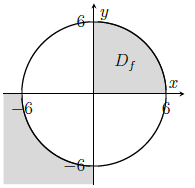
\includegraphics[scale=0.6]{pictures/3_4_a}
\end{center}
\item 
\begin{center}
	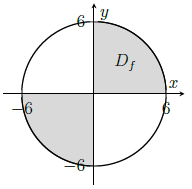
\includegraphics[scale=0.6]{pictures/3_4_b}
\end{center}
\item
\begin{center}
	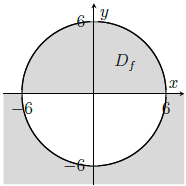
\includegraphics[scale=0.6]{pictures/3_4_c}
\end{center}
\item
\begin{center}
	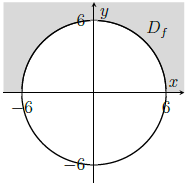
\includegraphics[scale=0.6]{pictures/3_4_d}
\end{center}
\end{enumerate}
\ \\
\subsection*{\frage{5}{3}}
Welche der folgenden Funktionen gehört zur unten dargestellten Fläche?\\
\begin{center}
	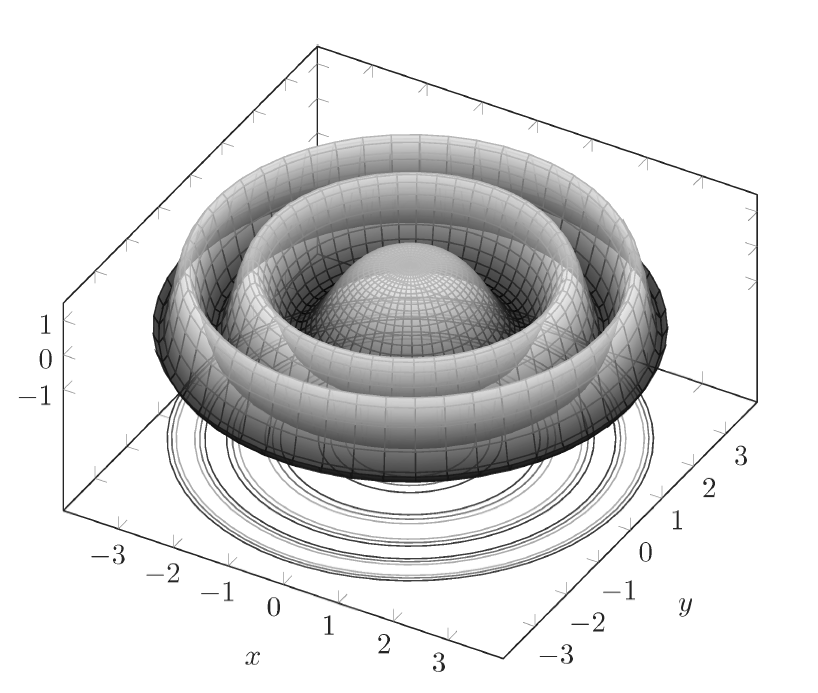
\includegraphics[scale=0.5]{pictures/3_5}
\end{center}
\renewcommand{\labelenumi}{(\alph{enumi})}
\begin{enumerate}
\item 
$ z = f_1(x,y) = e^{-(x+y^2)} $.
\item
$ z = f_2(x,y) = e^{x} e^y $.
\item
$ z = f_3(x,y) = e^{2 -x^2 +y^2}  $.
\item
$ z = f_4(x,y) = \cos(x^2 +y^2) $.
\item
$ z = f_5(x,y) = 2^{-(x + y^2)} $.
\item
$ z = f_6(x,y) = \sin(x+y) $.
\end{enumerate}
\ \\
\subsection*{\frage{6}{4}}
Wir betrachten die Cobb-Douglas Produktionsfunktion
\begin{align*}
	P(K,A) 
	=
	4 K^{0.25} A^{0.75} \ \ (K,A > 0).
\end{align*}
Für welchen Punkt $ (K_0, A_0) $ auf der Isoquante (Niveaulinie) $ P(K,A) = 64 $ ist die technische Substitutionsrate (des Faktors Arbeit $ A $ bezüglich des Faktors $ K $) gleich $ - \frac{1}{3} $ ?
\renewcommand{\labelenumi}{(\alph{enumi})}
\begin{enumerate}
	\item 
	$ (K_0, A_0) = ( 8 \sqrt{2}, 8 ) $.
	\item
	$ (K_0, A_0) = ( 8 , 16 )$.
	\item
	$ (K_0, A_0) = ( 32 , 32)$.
	\item
	$ (K_0, A_0) = ( 4 , 4\sqrt{2})$.
	\item
	$ (K_0, A_0) = ( 16 , 16\sqrt{2})$.
	\item
	$ (K_0, A_0) = ( 16 , 16)$.
\end{enumerate}
\ \\
\subsection*{\frage{7}{3}}
Gegeben ist die Funktion
\begin{align*}
	f(x,y) 
	=
	x^2 e^{\frac{x+y}{x}}
	-
	xy e^{\frac{x+y}{x-y}}
	+
	x \ln \left( \frac{x}{y} \right)
	\quad \textrm{für } x>0,y>0.
\end{align*}
Welche der folgenden Aussagen ist richtig?
\renewcommand{\labelenumi}{(\alph{enumi})}
\begin{enumerate}
	\item
	$ f  $ ist homogen vom Grad $ 0 $.
	\item
	$ f  $ ist homogen vom Grad $ 0.5 $.
	\item
	$ f $ ist linear homogen.	
	\item 
	$ f  $ ist homogen vom Grad $ 2 $.
	\item
	$ f $ ist nicht homogen.
\end{enumerate}
\ \\
\subsection*{\frage{8}{4}}
Gegeben ist die Funktion
\begin{align*}
	f(x,y)
	=
	\frac{x^{2a} y^b}{x^3 +y^3}
	- 
	\frac{1}{x^3 y^{3b} + x y^{2 + 3b}},
\end{align*}
wobei $ x > 0, y > 0 $ und $ a,b \in \R $.\\
\\
Für welche Werte von $ a $ und $ b $ gilt
\begin{align*}
	x f_x(x,y) + y f_y(x,y) = 0 \ \textrm{für alle } x>0, y>0\textrm{?}
\end{align*}
\renewcommand{\labelenumi}{(\alph{enumi})}
\begin{enumerate}
	\item 
	$a = 2$ und $ b=-1 $.
	\item
	$a = 1$ und $ b=1 $.
	\item
	$a = 1$ und $ b=-1 $.
	\item
	$a = 3$ und $ b=-2 $.
	\item
	$a = -2$ und $ b=1 $.
	\item
	Es gibt keine Werte $ a $ und $ b $, die die Bedingung erfüllen.
\end{enumerate}
\newpage
\section*{\hfil Lösungen \hfil}
\vspace{1cm}
\fancyhead[C]{\normalsize\textbf{$\qquad$ Teil I: Offene Aufgaben}}
\renewcommand{\labelenumi}{\theenumi.}
\section*{Aufgabe 1 (38 Punkte)}
\vspace{0.4cm}
%\titleformat{\subsection}[runin]
%{\normalfont\large\bfseries}{\thesubsection}{1em}{}
\subsection*{\aufgabe{a1}{8}} 
Die Wirtschaftsredakteurin eines wichtigen Verlagshauses zieht in Betracht,
kostenlose Exemplare eines Buchs an Dozierende der Wirtschaftswissenschaften an Schweizer Hochschulen zu verschicken, da sie weiss, dass Dozierende dazu neigen, Bücher als Kurslektüre auszuwählen, die sie bereits in ihren Regalen stehen haben. Die Fixkosten dieser Werbekampagne belaufen sich auf $100'000$ Schweizer Franken.
Die Stückkosten eines einzelnen Buchs betragen $10$ Schweizer Franken, im Handel werden die Bücher schließlich für $40$ Schweizer Franken pro Exemplar verkauft.
Auf der Basis historischer Daten schätzt die Redakteurin, dass wenn $x$ Gratisexemplare versendet werden, ein Verkauf von insgesamt
\begin{align*}
	B(x) = 20'000 - 19'000 e^{-0.0002 x }
\end{align*}
Exemplaren des Buchs erzielt wird. \\
\\
Zeigen Sie, dass wenn die Produktion auf maximal $6'000$ Bücher beschränkt ist, es genau eine Menge $ x^\star \in (0, 6'000)$ an Gratisexemplaren gibt, bei der die Gesamtkosten genau durch den Umsatz gedeckt werden.
\
\\
\textbf{Lösung:}
\begin{mdframed}
\underline{\textbf{Vorgehensweise:}}
\renewcommand{\labelenumi}{\theenumi.}
\begin{enumerate}
\item 

\end{enumerate}
\end{mdframed}
\underline{1. }\\

 
\newpage

\subsection*{\aufgabe{a2}{8}}
Die Wirtschaftsredakteurin eines wichtigen Verlagshauses zieht in Betracht,
kostenlose Exemplare eines Buchs an Dozierende der Wirtschaftswissenschaften an Schweizer Hochschulen zu verschicken, da sie weiss, dass Dozierende dazu neigen, Bücher als Kurslektüre auszuwählen, die sie bereits in ihren Regalen stehen haben. Die Fixkosten dieser Werbekampagne belaufen sich auf $100'000$ Schweizer Franken.
Die Stückkosten eines einzelnen Buchs betragen $10$ Schweizer Franken, im Handel werden die Bücher schließlich für $40$ Schweizer Franken pro Exemplar verkauft.
Auf der Basis historischer Daten schätzt die Redakteurin, dass wenn $x$ Gratisexemplare versendet werden, ein Verkauf von insgesamt
\begin{align*}
	B(x) = 20'000 - 19'000 e^{-0.0002 x }
\end{align*}
Exemplaren des Buchs erzielt wird. Wenn die Produktion auf maximal $6'000$ Bücher beschränkt ist, gibt es genau eine Menge $ x^\star \in (0, 6'000)$ an Gratisexemplaren, bei der die Gesamtkosten genau durch den Umsatz gedeckt werden.\\
\\
Verwenden Sie eine Taylor-Approximation zweiter Ordnung im Punkt $x_0 = 750$, um eine Näherung für $x^\star$ zu finden.
\\
 \\
\textbf{Lösung:}
\begin{mdframed}
\underline{\textbf{Vorgehensweise:}}
\renewcommand{\labelenumi}{\theenumi.}
\begin{enumerate}
\item Bestimme das Taylorpolynom. 
\end{enumerate}
\end{mdframed}

\underline{1. Bestimme das Taylorpolynom}\\

\newpage
\subsection*{\aufgabe{b}{12}}
Anne und Robert haben gerade erfolgreich ihr Masterprogramm in Quantitativen
Methoden an der Universität St.Gallen abgeschlossen und sind nun dabei, ihre eigene
Firma AlgoTrade aufzubauen, die Machine Learning Algorithmen für den computergesteuerten Handel an Finanzmärkten entwickelt. Sie haben bereits viele vielversprechende Ideen, jedoch fehlt ihnen das Eigenkapital. Die anfänglichen Investitionen für den Kauf der IT-Infrastruktur und für die Entwicklung der Software belaufen sich auf $1'500'000$ Schweizer Franken.
Ein Risikokapitalgeber ist zu einem Investment in Höhe von $500'000$ Schweizer Franken bereit, verlangt aber im Gegenzug einen Anteil von $30 \%$ an der Firma.
Zusätzlich nehmen Anne und Robert am 1. Januar 2022 einen Kredit in Höhe von $1'000'000$ Schweizer Franken zu einem jährlichen Zinssatz von $2 \% $ auf.
Die Bank verlangt dabei, dass $40 \%$ des geschuldeten Betrags bis Ende 2026 über konstante Zahlungen $C$, fällig jeweils am Jahresende, zurückgezahlt sein muss.
\begin{enumerate}
	\item[(b1)] Fügen Sie die Ereignisse und Mittelflüsse dem Zeitstrahl hinzu.
	\item[(b2)] Berechnen Sie die Höhe der Ratenzahlung $C$.
\end{enumerate}
Bereits nach 3 Jahren ist AlgoTrade sehr erfolgreich und generiert beträchtliche Umsätze. Beginnend mit der nächsten Rückzahlung am 31. Dezember 2025 wollen Anne und Robert jeweils $180'000$ Schweizer Franken am Ende jedes Jahres solange zurückzahlen, bis die bestehende Restschuld komplett getilgt ist.
\begin{enumerate}
	\item[(b3)] Ergänzen Sie die Information am Zeitstrahl und berechnen Sie die Restschuld am 1. Januar 2025, also direkt nach der jüngsten Rückzahlung.
	\item[(b4)] Am 1. Januar 2029, direkt nach der jüngsten Rückzahlung, verkaufen Anne und Robert	ihre Firma für $5'000'000$ Schweizer Franken und tilgen mit ihrem Anteil die bestehende	Restschuld. Wie hoch ist ihr Gewinn?
\end{enumerate}
\begin{center}
	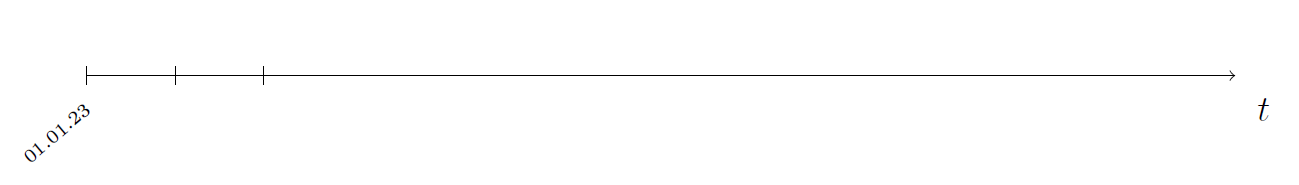
\includegraphics[scale=0.45]{pictures/zeitstrahl_1_b}
\end{center}
\ \\
\textbf{Lösung:}
\begin{mdframed}
\underline{\textbf{Vorgehensweise:}}
\begin{enumerate}
\item[(b1)] Füge den Kredit und die Raten zum Zeitstrahl hinzu.
\end{enumerate}
\end{mdframed}

\underline{(b1) }\\


\newpage
\subsection*{\aufgabe{c}{10}}
Information spielt in der Entscheidungsfindung eine wesentliche Rolle. Allerdings
sehen sich Unternehmen, wie wir erst kürzlich beobachten konnten, einem Zielkonflikt
ausgesetzt. Einerseits ermöglicht das Sammeln möglichst genauer privater Informationen eine verbesserte, massgeschneiderte Lösung für ihre Kunden (die zu einem höheren Preis verkauft werden kann), andererseits erhöht es den potentiellen Schaden, den sie ihren Kunden durch Datenschutzverletzungen (und sich selbst durch mögliche juristische Folgen) zufügen könnten.\\
\\
Sei $I \geq 0 $ die Menge an Informationen, die ein Unternehmen sammelt, und $b(I)$ der Nutzen für den Kunden hinsichtlich der angebotenen Dienstleistung oder des angebotenen Produktes. Wir nehmen an, dass:
\begin{align*}
	b(I)
	= 
	\begin{cases}
		0 &\quad \textrm{für } 0 \leq I  < I_0\\
		s \left( 1 - \frac{I_0}{I} \right) & \quad \textrm{für } I \geq I_0
	\end{cases}.
\end{align*}
Demnach ist $I_0 > 0 $ die Mindestmenge an Information, die benötigt wird, um einen Nutzen für den Kunden zu generieren, und der Nutzen ist durch $s > 0 $ beschränkt, d.h., der Nutzen wird nie grösser als $s$, egal wie viel Information gesammelt wird. Im Gegensatz dazu soll der erwartete Schaden durch eine Datenschutzverletzung durch
\begin{align*}
	d(I) = \frac{1}{2} q s I^2
\end{align*}
gegeben sein, wobei $q \in (0,1)$ die Wahrscheinlichkeit einer solchen Verletzung darstellt.
Zudem nehmen wir an, dass $q I_0^2 < \frac{8}{27}$ gilt. Für einen potentiellen Kunden ist die relevante Grösse der Trade-off $v(I)$ zwischen dem Nutzen $b(I)$ und dem möglichen Schaden $d(I)$, d.h., $v(I) = b(I) - d(I)$.\\
\\
Für welche Menge $I^\star \geq 0$ an Informationen erzielt der Kunde den bestmögliche Trade-off, d.h. den grössten Wert für $v$?
Bestimmen Sie die Antwort in Abhängigkeit der Parameter $s, I_0, q$.
Weisen Sie nach, dass $I^\star$ tatsächlich ein Maximum von $v$ ist.\\
\\
\textit{Hinweis:} Die Bedingung $q I_0^2 < \frac{8}{27}$ stellt sicher, dass $I^\star > I_0 $ gilt.\\
\\
\textbf{Lösung:}
\begin{mdframed}
\underline{\textbf{Vorgehensweise:}}
\begin{enumerate}
\item[(c1)] 
\end{enumerate}
\end{mdframed}

\underline{(c1) }\\





%\fancyhead[C]{\normalsize\textbf{$\qquad$ Teil II: Multiple-Choice}}
\section*{Aufgabe 2 (32 Punkte)}
\vspace{0.4cm}
\subsection*{\frage{1}{4}}
Die Funktion $ f(x,y) \ = \ (x-2)^2 -y^2 $ hat einen Sattelpunkt beim Punkt $ P \ = \ (2,0) $. Welche der folgenden Aussagen ist korrekt?
\renewcommand{\labelenumi}{(\alph{enumi})}
\begin{enumerate}
	\item Die Funktion $ f $ hat unter der Nebenbedingung $ 2x \ - y \ - \ 4 \ = \ 0 $ ein lokales Minimum beim Punkt $ P $.
	\item Die Funktion $ f $ hat unter der Nebenbedingung $ 2x \ - y \ - \ 4 \ = \ 0 $ einen Sattelpunkt beim Punkt $ P $.
	\item Die Funktion $ f $ hat unter der Nebenbedingung $ -x \ - 2y \ - \ 4 \ = \ 0 $ einen Sattelpunkt beim Punkt $ P $.
	\item Die Funktion $ f $ hat unter der Nebenbedingung $ -\frac{1}{2}x \ - y \ + \ 1 \ = \ 0 $ ein lokales Minimum beim Punkt $ P $.
	\item Die Funktion $ f $ hat unter der Nebenbedingung $ -\frac{1}{2}x \ - y \ + \ 1 \ = \ 0 $ ein lokales Maximum beim Punkt $ P $.
\end{enumerate}
\ \\
\textbf{Lösung:}
\begin{mdframed}
\underline{\textbf{Vorgehensweise:}}
\renewcommand{\labelenumi}{\theenumi.}
\begin{enumerate}
\item 
\end{enumerate}
\end{mdframed}

\underline{1. }\\


\newpage

\subsection*{\frage{2}{3}}
Sei $ f \ : \ D_f \to \mathbb{R} $ eine positive Funktion zweier reeller Variablen, welche ein lokales Maximum beim Punkt $ P = (5,2)  $ hat.
Sei $ h  \ : \ D_f \to \mathbb{R} $ die Funktion definiert durch
\begin{align*}
	h(x,y) = e^{\sqrt{f(x,-y)}}.
\end{align*} 
Welche der folgenden Aussagen ist korrekt?
\renewcommand{\labelenumi}{(\alph{enumi})}
\begin{enumerate}
	\item Die Funktion $ h $ hat ein lokales Maximum beim Punkt $ Q = (-5,2). $
	\item Die Funktion $ h $ hat ein lokales Maximum beim Punkt $ Q = (5,-2). $
	\item Die Funktion $ h $ hat ein lokales Minimum beim Punkt $ Q = (-5,2). $
	\item Die Funktion $ h $ hat ein lokales Minimum beim Punkt $ Q = (5,-2). $
	\item Wir können die Extremstellen von $ h $ nicht analysieren, ohne mehr Informationen zur Funktion $ f $ zu haben.
\end{enumerate}
\ \\
\textbf{Lösung:}
\begin{mdframed}
	\underline{\textbf{Vorgehensweise:}}
	\renewcommand{\labelenumi}{\theenumi.}
	\begin{enumerate}
		\item 
	\end{enumerate}
\end{mdframed}
\underline{1. }\\

\newpage
\subsection*{\frage{3}{3}}
Sei $ F $ die Stammfunktion der stetigen Funktion $ f $ einer reellen Variable $ x $ und sei $ g $ eine lineare Funktion, d.h. $ g(x) = ax +b $ für die Parameter $ a,b \in \mathbb{R} $. Das unbestimmte Integral
\begin{align*}
	\int f(x) g(x) \ dx.
\end{align*}
ist gleich:
\renewcommand{\labelenumi}{(\alph{enumi})}
\begin{enumerate}
	\item 
	$ a x F(x) + b F(x) - a \int F(x) dx$.
	\item 
	$ g(x) F(x) - a \int f(x) dx$.
	\item 
	$ \left(\frac{1}{2} a x^2 +b x\right) F(x) - \int a F(x) dx$.
	\item
	$ \left(\frac{1}{2} a x^2 +b x\right) F(x) - \int  F(x) g(x) dx$.
	\item 
	Wir können das Integral nicht transformieren, ohne mehr Informationen zur Funktion $ f $ zu haben.
\end{enumerate}
\ \\
\textbf{Lösung:}
\begin{mdframed}
\underline{\textbf{Vorgehensweise:}}
\renewcommand{\labelenumi}{\theenumi.}
\begin{enumerate}
\item 
\end{enumerate}
\end{mdframed}

\underline{1. }\\


\newpage

\subsection*{\frage{4}{3}}
Sei $ f $ eine \textit{gerade} Funktion, welche die folgenden (Integral-) Gleichungen erfüllt:
\begin{align*}
	\int_{2}^3 f(x) \ dx = 10, \ \textrm{und} \
	\int_1^3 f(x) \ dx = 15.
\end{align*}
Das bestimmte Integral
\begin{align*}
	\int_{-2}^{-1} (2 - f(x) ) \ dx
\end{align*}  
gleich
\renewcommand{\labelenumi}{(\alph{enumi})}
\begin{enumerate}
	\item 
	$ -1 $.
	\item
	$ -2 $.
	\item
	$ -3 $.
	\item
	$ -4 $.
	\item
	Wir haben nicht genügend Informationen, um diesen Wert auszurechnen.
\end{enumerate}
\ \\
\textbf{Lösung:}
\begin{mdframed}
\underline{\textbf{Vorgehensweise:}}
\renewcommand{\labelenumi}{\theenumi.}
\begin{enumerate}
\item Forme das Integral um und verwende, dass die Funktion gerade ist.
\end{enumerate}
\end{mdframed}

\underline{1. Forme das Integral um und verwende, dass die Funktion gerade ist}\\
Mit der Information, dass $f$ gerade ist und den gegebenen Werten für das Integral gilt:
\begin{align*}
	\int_{-2}^{-1} (2 - f(x) ) \ dx
	&=
	\int_{-2}^{-1} 2  \ dx
	-
	\int_{-2}^{-1} f(x) \ dx
	\underset{f \ \text{gerade}}{=}
	2
	-
	\int_{1}^{2} f(x) \ dx\\
	&=
	2 
	-
	\left(\int_{1}^{3} f(x) \ dx - \int_{2}^{3} f(x) \ dx\right)
	=
	2
	-
	(15 - 10)
	=-3
\end{align*}
Damit ist die Antwort (c) korrekt.

\newpage
\subsection*{\frage{5}{4}}
Gegeben seien die Matrizen $ A_{n \times m} $ und $ B_{m \times n} $ für $ m,n \in \mathbb{N} $.\\
\\
Es folgt:
\renewcommand{\labelenumi}{(\alph{enumi})}
\begin{enumerate}
	\item 
	Die Matrix $ (AB)^\top $ hat die Dimensionen $ n \times m $.
	\item 
	Die Matrix $ (AB)^\top $ ist symmetrisch, falls $ A $ symmetrisch ist.
	\item 
	Die Matrix $ (AB)^\top $ ist invertierbar, falls $ \mathrm{rg}(A) = \mathrm{rg}(B) = n $.
	\item 
	Die Matrix $ (AB)^\top $ ist invertierbar, falls $ BA $ invertierbar ist.
	\item 
	Die Matrix $ (AB)^\top $ ist invertierbar, falls sie $ n $ reelle Eigenwerte besitzt, welche ungleich null sind.
\end{enumerate}
\ \\
\textbf{Lösung:}
\begin{mdframed}
\underline{\textbf{Vorgehensweise:}}
\renewcommand{\labelenumi}{\theenumi.}
\begin{enumerate}
\item Schließe falsche Antworten aus.
\end{enumerate}
\end{mdframed}

\underline{1. Schließe falsche Antworten aus}\\
Das Produkt $AB$ ist eine $(n \times n)$ Matrix. 
Somit gilt dies auch für $(AB)^\top$. Also ist Antwort (a) nur korrekt, falls $n = m$ ist und gilt nicht im Allgemeinen.
Für die Antwort (b) geben wir ein Gegenbeispiel an:
\begin{align*}
	A
	= 
	\begin{pmatrix}
		1 & 0\\
		0 & 1
	\end{pmatrix},
	\
	B
	=
	\begin{pmatrix}
		1 & 1 \\
		0 & 1
	\end{pmatrix}
	\
	\Rightarrow
	\
	(AB)^\top
	= 
	\begin{pmatrix}
		1 & 0\\
		1 & 1
	\end{pmatrix}.
\end{align*}
Auch für die Antwort (c) finden wir ein Gegenbeispiel. Hierbei nutzen wir aus, dass $A$ und $B$ nicht quadratisch sein müssen:
\begin{align*}
	A
	=
	\begin{pmatrix}
		1 & 0 & 0 & 0\\
		0 & 1 & 0 & 0
	\end{pmatrix},
	\
	B =
	\begin{pmatrix}
		0 & 0 \\
		0 & 0 \\
		1 & 0 \\
		0 & 1
	\end{pmatrix}
	\
	\Rightarrow
	\
	(AB)^\top = 
	\begin{pmatrix}
		0 & 0 \\
		0 & 0
	\end{pmatrix}
\end{align*}
Es gilt $\mathrm{rg}(A) = \mathrm{rg}(B) = 2 = n$ und $\mathrm{rg}\left((AB)^\top\right) = 0$, womit $(AB)^\top$ nicht invertierbar ist.\\
Zur Antwort (d): Falls $AB$ invertierbar ist, gilt dies wegen
\begin{align*}
	\left((AB)^\top\right)^{-1} = \left((AB)^{-1}\right)
\end{align*}
Wenn $n = m $ gelten würde, wäre (d) wegen 
\begin{align*}
	\det(BA) = \det(B) \det(A) \neq 0
\end{align*}
korrekt. Für $n \neq m$ gilt dies nicht, da die Matrixmultiplikation nicht kommutativ ist. Dies lässt sich auch durch ein Gegenbeispiel untermauern:
\begin{align*}
	B
	=
	\begin{pmatrix}
		1 & 0 & 0 \\
		0 & 1 & 0
	\end{pmatrix},
	\
	A 
	=
	\begin{pmatrix}
		1 & 0 \\
		0 & 1\\
		0 & 0
	\end{pmatrix}
	\ \Rightarrow \
	BA=
	\begin{pmatrix}
		1 & 0\\
		0 & 1
	\end{pmatrix}, \
	AB =
	\begin{pmatrix}
		1 & 0 & 0\\
		0 & 1 & 0\\
		0 & 0 & 0
	\end{pmatrix}.
\end{align*}
$BA$ ist invertierbar, $AB$ jedoch nicht.\\
\\
Somit bleibt die Anwort (e) als korrekte Antwort übrig.
In der Tat gilt diese Aussage für jede quadratische Matrix,
da der Rang einer quadratischen Matrix für jeden Eigenwert ungleich $0$ um eins anwächst. Somit gilt $\mathrm{rg}\left((AB)^\top\right) = n$ und $(AB)^\top $ ist invertierbar.\\
\\
Damit ist Antwort (e) korrekt.
\newpage

\subsection*{\frage{6}{3}}
Gegeben sei die $ (n \times n ) $-dimensionale, reguläre Matrix $ A $ mit einem reellen Eigenwert $ \lambda \neq 0 $.\\
\\
Es folgt, dass die Matrix
\begin{align*}
	A^{-4} = A^{-1} \cdot A^{-1} \cdot A^{-1} \cdot A^{-1}
\end{align*}
den folgenden Eigenwert hat:
\renewcommand{\labelenumi}{(\alph{enumi})}
\begin{enumerate}
	\item 
	$ \frac{1}{\lambda^4} $.
	\item 
	$ \frac{4}{\lambda} $.
	\item
	$ \lambda$.
	\item
	$\lambda^3 $.
	\item 
	Es ist nicht möglich, eine Aussage bezüglich der Eigenwerte von $ A^{-4} $ zu treffen.
\end{enumerate}
\ \\
\textbf{Lösung:}
\begin{mdframed}
\underline{\textbf{Vorgehensweise:}}
\renewcommand{\labelenumi}{\theenumi.}
\begin{enumerate}
\item Verwende die Definition des Eigenwerts.
\end{enumerate}
\end{mdframed}

\underline{1. Verwende die Definition des Eigenwerts}\\
Sei $ \lambda  $ der Eigenwert der regulären Matrix $ A $ und $ \textbf{v} $ ein zugehöriger Eigenvektor. Dann gilt:
\begin{align*}
	A \cdot  \textbf{v} = \lambda \textbf{v}
	\ \Leftrightarrow \
	A^{-1} \cdot A \textbf{v} = I \cdot \textbf{v} = \textbf{v} = A^{-1} \cdot \lambda \textbf{v}
	\ \Leftrightarrow \
	A^{-1} \cdot \textbf{v} = \frac{1}{\lambda} \textbf{v}.
\end{align*} 
Somit ist $ \frac{1}{\lambda} $ ein Eigenwert von $ A^{-1} $.\\
\\
\textit{Hinweis}: Wegen $ \det(A) \neq  0 $ kann $ 0 $ kein Eigenwert einer regulären Matrix sein.\\
\\
Wegen
\begin{align*}
	A^{-4} \cdot \textbf{v} 
	= 
	A^{-1} \cdot A^{-1} \cdot A^{-1} \cdot A^{-1} \cdot  \textbf{v}
	=
	A^{-1} \cdot A^{-1} \cdot A^{-1} \cdot \frac{1}{\lambda} \textbf{v}
	=
	...
	=
	\frac{1}{\lambda^4} \textbf{v}  
\end{align*}
ist $ \frac{1}{\lambda^4} $ ein Eigenwert von $ A^{-4} $.\\
\\
Damit ist die Antwort (a) korrekt.


\newpage
\subsection*{\frage{7}{3}}
Gegeben sei das lineare Gleichungssystem
\begin{align*}
	A \textbf{x} = \textbf{b}.
\end{align*}
\textit{Keine} notwendige Annahme, um das lineare Gleichungssystem mithilfe der Cramerschen Regel zu lösen zu können, ist:
\renewcommand{\labelenumi}{(\alph{enumi})}
\begin{enumerate}
	\item 
	$ A $ ist quadratisch.
	\item
	$ A $ hat vollen Rang.
	\item
	$ \det(A) \neq 0$.
	\item
	$ \textbf{b} \neq \textbf{0} $.
	\item
	$ \mathrm{rg}(A) = \mathrm{rg}([A,\textbf{b}])$.
\end{enumerate}
\ \\
\textbf{Lösung:}
\begin{mdframed}
\underline{\textbf{Vorgehensweise:}}
\renewcommand{\labelenumi}{\theenumi.}
\begin{enumerate}
\item Nutze den Quotienten aus Determinanten der Cramerschen Regel.
\end{enumerate}
\end{mdframed}

\underline{1. Nutze den Quotienten aus Determinanten der Cramerschen Regel}\\
Ein Komponente $ x_i $ des Lösungsvektors wird mit der Cramerschen Regel durch
\begin{align*}
	x_i = \frac{\det(A_i)}{\det(A)}
\end{align*}
bestimmt. Da ist $ \det(A)  $ im Nenner vorkommt, ist $ \det(A) \neq 0 $ notwendig um die Cramersche Regel anzuwenden.
Determinanten sind nur für quadratische Matrizen definiert, womit $ A $ quadratisch sein muss.
Wegen $ \det(A) \neq 0 $ muss $ A $ invertierbar sein. Für quadratische Matrizen ist dies äquivalent zu einem vollem Rang. Der volle Rang wiederum ist äquivalent dazu, dass $ \mathrm{rg}(A) = \mathrm{rg}([A,\textbf{b}]) $ gilt.
Damit haben wir festgestellt, dass für die Cramersche Regel die Annahmen (a), (b), (c) und (e) notwendig sind.\\
\\
Damit ist Antwort (d) korrekt.\\
\\
Die Annahme $ \textbf{b} \neq \textbf{0} $ ist nicht notwendig. Für den Nullvektor würde man mit der Cramerschen Regel eben auch den Nullvektor als Lösung erhalten. 
\newpage

\subsection*{\frage{8}{3}}
Sei $ A $ eine $ (1 \times 5) $-Matrix definiert als
\begin{align*}
	A
	=
	\left(
	\textbf{a}_1,
	\textbf{a}_2,
	\textbf{a}_3,
	\textbf{a}_4,
	\textbf{a}_5
	\right).
\end{align*}
für $ a_i \in \mathbb{R}, \ i = 1,2,...,5 $.\\
\\
Es folgt, dass:
\renewcommand{\labelenumi}{(\alph{enumi})}
\begin{enumerate}
	\item 
	$ \mathrm{rg}(A) = 5 $, falls $ a_i \neq 0 $ für alle $ i \in \{1,2,3,4,5\} $ und $ a_i \neq a_j $ für $ i \neq j $.
	\item
	$ \mathrm{rg}(A) = 5 $, falls $ a_i \neq 0 $ für mindestens ein $ i \in \{1,2,3,4,5\} $.
	\item
	$ \mathrm{rg}(A) = 1 $, falls $ a_i \neq 0 $ für mindestens ein $ i \in \{1,2,3,4,5\} $.
	\item
	$ \mathrm{rg}(A) = 0 $, falls $ a_i = 0 $ für genau ein $ i \in \{1,2,3,4,5\} $.
	\item
	$1 <  \mathrm{rg}(A)\leq 5 $, falls $ a_i \neq 0 $ für mindestens ein $ i \in \{1,2,3,4,5\} $.
	\item 
	Es ist nicht möglich, mit den gegebenen Informationen eine Aussage zum Rang von $ A $ zu machen.
\end{enumerate}
\ \\
\textbf{Lösung:}
\begin{mdframed}
\underline{\textbf{Vorgehensweise:}}
\renewcommand{\labelenumi}{\theenumi.}
\begin{enumerate}
\item Verwende die Definition des Ranges.
\end{enumerate}
\end{mdframed}

\underline{1. Verwende die Definition des Ranges}\\
Der Rang einer Matrix $ A $ ist definiert durch
\begin{align*}
	\mathrm{rg}(A) := \ \text{Anzahl der linear unabhängigen Spalten von $ A $}.
\end{align*}
Da $ A $ eine $ (1 \times 5) $ Matrix ist, sind die einzelnen Spalten Skalare.
Damit kann der Rang höchstens $ 1 $ sein und ist genau dann $ 1 $, wenn mindestens einer dieser Skalare ungleich $ 0 $ ist.\\
\\
Also ist die Antwort (c) korrekt.\\
\\
Man kann den Rang einer Matrix auch als die Anzahl der linear unabhängigen Zeilen definieren. Diese ist äquivalent zu der Definition über die linear unabhängigen Spalten. Sei $ \textbf{v} := A^\top $ der Zeilenvektor von $ A $. Die Definition der lineare Unabhängigkeit über einen Vektor ist: 
\begin{align*}
	\lambda \textbf{v} = \textbf{0} \ \Rightarrow \ \lambda = 0.
\end{align*}
Diese kann nur erfüllt sein, falls mindestens ein Eintrag von $ \textbf{v} $ ungleich $ 0 $ ist. 


\newpage
\subsection*{\frage{9}{3}}
Sei $ A $ eine $ (4 \times 2) $-dimensionale Matrix mit Rang $ 2 $ und $ B $ eine Matrix mit den Dimensionen $ (4 \times 3) $ mit Rang $ 1 $.\\
\\
Wir definieren die Matrix $ C $ als die Aneinanderreihung der Spalten von $ A $ und $ B $ wie folgt:
\begin{align*}
	C = [A, B, A].
\end{align*}
Es folgt, dass:
\renewcommand{\labelenumi}{(\alph{enumi})}
\begin{enumerate}
	\item 
	$ \mathrm{rg}(C) = 2 $.
	\item
	$ \mathrm{rg}(C) = 3 $.
	\item
	$ \mathrm{rg}(C)\in \{2,3\} $.
	\item
	$ \mathrm{rg}(C) = 4 $.
	\item
	Die gegebenen Informationen sind nicht ausreichend, um eine Aussage über den Rang von $ C $ treffen zu können.
\end{enumerate}
\ \\
\textbf{Lösung:}
\begin{mdframed}
	\underline{\textbf{Vorgehensweise:}}
	\renewcommand{\labelenumi}{\theenumi.}
	\begin{enumerate}
		\item Verwende die Definition des Ranges.
	\end{enumerate}
\end{mdframed}

\underline{1. Verwende die Definition des Ranges}\\
Der Rang der Matrix $ C $ ist definiert durch
\begin{align*}
	\mathrm{rg}(C) := \ \text{Anzahl der linear unabhängigen Spalten von $ C $}.
\end{align*}
Die Matrix $ C $ hat die Dimension $ (4 \times 7) $. Die Spalten von $ A $ treten doppelt auf. Damit tragen von $ A $ zwei Spalten und von $ B $ eine Spalte zu dem Rang von $ C $ bei. Durch elementare Spaltenoperationen gilt:
\begin{align*}
	C = \begin{pmatrix}
		\textbf{a}_1 \ \textbf{a}_2  \
		\textbf{b}_1  \ \textbf{b}_2 \ \textbf{b}_3 \
		\textbf{a}_1  \ \textbf{a}_2
	\end{pmatrix}
\leadsto
	\begin{pmatrix}
		\textbf{a}_1 \ \textbf{a}_2 \ 
		\tilde{\textbf{b}_1} \ \textbf{0} \  \textbf{0} \
		\textbf{0} \ \textbf{0}
	\end{pmatrix}
\end{align*}
Hierbei sind $ \textbf{a}_i $, $ i = 1,2 $ und $ \textbf{b}_i $, $ i = 1,2,3 $ die Spaltenvektoren von $ A $ und $ B $ und $ \tilde{\textbf{b}_1} $ der aus den Spaltenoperationen entstehende Spaltenvektor. 
Da $ \textbf{a}_1 $ und $ \textbf{a}_2 $ linear unabhängig sind, beträgt der Rang von $ C $ mindestens $ 2 $. Der Rang von $ C $ ist $ 3 $, falls sich $ \tilde{\textbf{b}_1} $ nicht von $ \textbf{a}_1 $ und $ \textbf{a}_2 $ linear kombinieren lässt, d.h. die Vektoren $ \textbf{a}_1 $, $ \textbf{a}_2 $ und $ \tilde{\textbf{b}_1} $ sind linear unabhängig.\\
\\
Damit ist die Antwort (c) korrekt.

\newpage
\subsection*{\frage{10}{3}}
Sei $ A \in \mathbb{R}^{n\times n} $ eine quadratische obere Dreiecksmatrix, d.h. eine quadratische Matrix deren Elemente unterhalb der Diagonale null sind.\\
\\
Welche der folgenden Aussagen ist \textit{nicht} korrekt bezüglich der Matrix $ A $?
\renewcommand{\labelenumi}{(\alph{enumi})}
\begin{enumerate}
	\item 
	Die Determinante ist das Produkt der Elemente auf der Diagonale.
	\item
	Die Matrix $ A + A^\top $ ist symmetrisch.
	\item
	Falls die Inverse $ A^{-1} $ existiert, so ist sie ebenfalls eine obere Dreiecksmatrix.
	\item
	Die Eigenwerte von $ A $ entsprechen den Elementen auf der Diagonale
	\item 
	Die Eigenvektoren von $ A $ entsprechen den Zeilen von $ A $.
\end{enumerate}
\ \\
\textbf{Lösung:}
\begin{mdframed}
	\underline{\textbf{Vorgehensweise:}}
	\renewcommand{\labelenumi}{\theenumi.}
	\begin{enumerate}
		\item Schließe falsche Antworten aus.
	\end{enumerate}
\end{mdframed}

\underline{1. Schließe falsche Antworten aus}\\
Um die richtige Antwort zu finden, stellen wir fest welche Aussagen korrekt sind.\\
\\
Die Aussage (a) folgt direkt aus dem Laplaceschen Entwicklungssatz. Um die Eigenwerte von $A$ zu bestimmen lösen wir $\det(A - \lambda I) = 0$. Da $A$ eine obere Dreiecksmatrix ist, gilt dies auch für $A - \lambda I$. Dementsprechend gilt
\begin{align*}
	\det(A - \lambda I)
	=(a_{11} - \lambda) \cdot (a_{22} - \lambda) \cdots (a_{nn} - \lambda)
\end{align*}
mit dem Laplaceschen Entwicklungssatz. Die Nullstellen (also Eigenwerte) entsprechen den Elementen auf der Diagonale womit die Aussage (d) korrekt ist.
Die Aussage (b) gilt wegen
\begin{align*}
	(A + A^\top)^\top 
	= A^\top + \left( A^\top \right)^\top  
	= A + A^\top,
\end{align*}
d.h. obige Addition erzwingt für alle $(n \times n)$ Matrizen die Symmetrieeigenschaft $B = B^\top$.
Die Antwort (c) ist korrekt, da bei einer Matrixmultiplikation mit einer oberern Dreiecksmatrix auch nur diejenigen Elemente zum Ergebnis beitragen, welche auf oder oberhalb der Diagonalen liegen. Alternativ kann man sich hierfür überlegen, welche elementaren Zeilenoperationen bei der Bestimmung der inversen Matrix notwendig sind.\\
\\
Somit bleibt nur die Antwort (e) übrig. Diese Aussage ist in der Tat nicht korrekt.
Wir betrachten
\begin{align*}
	A =
	\begin{pmatrix}
		1 & 1 \\
		0 & 2
	\end{pmatrix}.
\end{align*}
Diese obere Dreiecksmatrix hat die Eigenwerte $1$ und $2$ mit den Eigenvektoren
\begin{align*}
	\begin{pmatrix}
		1\\
		0
	\end{pmatrix}
	\ \text{und} \
	\begin{pmatrix}
		1\\
		1
	\end{pmatrix}.
\end{align*}
Dies ist ein Gegenbeispiel, womit Antwort (e) korrekt ist.

\newpage
\fancyhead[C]{\normalsize\textbf{$\qquad$ Teil II: Multiple-Choice}}
\section*{Aufgabe 2 (32 Punkte)}
\vspace{0.4cm}
\subsection*{\frage{1}{4}}
Die Funktion $ f(x,y) \ = \ (x-2)^2 -y^2 $ hat einen Sattelpunkt beim Punkt $ P \ = \ (2,0) $. Welche der folgenden Aussagen ist korrekt?
\renewcommand{\labelenumi}{(\alph{enumi})}
\begin{enumerate}
	\item Die Funktion $ f $ hat unter der Nebenbedingung $ 2x \ - y \ - \ 4 \ = \ 0 $ ein lokales Minimum beim Punkt $ P $.
	\item Die Funktion $ f $ hat unter der Nebenbedingung $ 2x \ - y \ - \ 4 \ = \ 0 $ einen Sattelpunkt beim Punkt $ P $.
	\item Die Funktion $ f $ hat unter der Nebenbedingung $ -x \ - 2y \ - \ 4 \ = \ 0 $ einen Sattelpunkt beim Punkt $ P $.
	\item Die Funktion $ f $ hat unter der Nebenbedingung $ -\frac{1}{2}x \ - y \ + \ 1 \ = \ 0 $ ein lokales Minimum beim Punkt $ P $.
	\item Die Funktion $ f $ hat unter der Nebenbedingung $ -\frac{1}{2}x \ - y \ + \ 1 \ = \ 0 $ ein lokales Maximum beim Punkt $ P $.
\end{enumerate}
\ \\
\textbf{Lösung:}
\begin{mdframed}
\underline{\textbf{Vorgehensweise:}}
\renewcommand{\labelenumi}{\theenumi.}
\begin{enumerate}
\item 
\end{enumerate}
\end{mdframed}

\underline{1. }\\


\newpage

\subsection*{\frage{2}{3}}
Sei $ f \ : \ D_f \to \mathbb{R} $ eine positive Funktion zweier reeller Variablen, welche ein lokales Maximum beim Punkt $ P = (5,2)  $ hat.
Sei $ h  \ : \ D_f \to \mathbb{R} $ die Funktion definiert durch
\begin{align*}
	h(x,y) = e^{\sqrt{f(x,-y)}}.
\end{align*} 
Welche der folgenden Aussagen ist korrekt?
\renewcommand{\labelenumi}{(\alph{enumi})}
\begin{enumerate}
	\item Die Funktion $ h $ hat ein lokales Maximum beim Punkt $ Q = (-5,2). $
	\item Die Funktion $ h $ hat ein lokales Maximum beim Punkt $ Q = (5,-2). $
	\item Die Funktion $ h $ hat ein lokales Minimum beim Punkt $ Q = (-5,2). $
	\item Die Funktion $ h $ hat ein lokales Minimum beim Punkt $ Q = (5,-2). $
	\item Wir können die Extremstellen von $ h $ nicht analysieren, ohne mehr Informationen zur Funktion $ f $ zu haben.
\end{enumerate}
\ \\
\textbf{Lösung:}
\begin{mdframed}
	\underline{\textbf{Vorgehensweise:}}
	\renewcommand{\labelenumi}{\theenumi.}
	\begin{enumerate}
		\item 
	\end{enumerate}
\end{mdframed}
\underline{1. }\\

\newpage
\subsection*{\frage{3}{3}}
Sei $ F $ die Stammfunktion der stetigen Funktion $ f $ einer reellen Variable $ x $ und sei $ g $ eine lineare Funktion, d.h. $ g(x) = ax +b $ für die Parameter $ a,b \in \mathbb{R} $. Das unbestimmte Integral
\begin{align*}
	\int f(x) g(x) \ dx.
\end{align*}
ist gleich:
\renewcommand{\labelenumi}{(\alph{enumi})}
\begin{enumerate}
	\item 
	$ a x F(x) + b F(x) - a \int F(x) dx$.
	\item 
	$ g(x) F(x) - a \int f(x) dx$.
	\item 
	$ \left(\frac{1}{2} a x^2 +b x\right) F(x) - \int a F(x) dx$.
	\item
	$ \left(\frac{1}{2} a x^2 +b x\right) F(x) - \int  F(x) g(x) dx$.
	\item 
	Wir können das Integral nicht transformieren, ohne mehr Informationen zur Funktion $ f $ zu haben.
\end{enumerate}
\ \\
\textbf{Lösung:}
\begin{mdframed}
\underline{\textbf{Vorgehensweise:}}
\renewcommand{\labelenumi}{\theenumi.}
\begin{enumerate}
\item 
\end{enumerate}
\end{mdframed}

\underline{1. }\\


\newpage

\subsection*{\frage{4}{3}}
Sei $ f $ eine \textit{gerade} Funktion, welche die folgenden (Integral-) Gleichungen erfüllt:
\begin{align*}
	\int_{2}^3 f(x) \ dx = 10, \ \textrm{und} \
	\int_1^3 f(x) \ dx = 15.
\end{align*}
Das bestimmte Integral
\begin{align*}
	\int_{-2}^{-1} (2 - f(x) ) \ dx
\end{align*}  
gleich
\renewcommand{\labelenumi}{(\alph{enumi})}
\begin{enumerate}
	\item 
	$ -1 $.
	\item
	$ -2 $.
	\item
	$ -3 $.
	\item
	$ -4 $.
	\item
	Wir haben nicht genügend Informationen, um diesen Wert auszurechnen.
\end{enumerate}
\ \\
\textbf{Lösung:}
\begin{mdframed}
\underline{\textbf{Vorgehensweise:}}
\renewcommand{\labelenumi}{\theenumi.}
\begin{enumerate}
\item Forme das Integral um und verwende, dass die Funktion gerade ist.
\end{enumerate}
\end{mdframed}

\underline{1. Forme das Integral um und verwende, dass die Funktion gerade ist}\\
Mit der Information, dass $f$ gerade ist und den gegebenen Werten für das Integral gilt:
\begin{align*}
	\int_{-2}^{-1} (2 - f(x) ) \ dx
	&=
	\int_{-2}^{-1} 2  \ dx
	-
	\int_{-2}^{-1} f(x) \ dx
	\underset{f \ \text{gerade}}{=}
	2
	-
	\int_{1}^{2} f(x) \ dx\\
	&=
	2 
	-
	\left(\int_{1}^{3} f(x) \ dx - \int_{2}^{3} f(x) \ dx\right)
	=
	2
	-
	(15 - 10)
	=-3
\end{align*}
Damit ist die Antwort (c) korrekt.

\newpage
\subsection*{\frage{5}{4}}
Gegeben seien die Matrizen $ A_{n \times m} $ und $ B_{m \times n} $ für $ m,n \in \mathbb{N} $.\\
\\
Es folgt:
\renewcommand{\labelenumi}{(\alph{enumi})}
\begin{enumerate}
	\item 
	Die Matrix $ (AB)^\top $ hat die Dimensionen $ n \times m $.
	\item 
	Die Matrix $ (AB)^\top $ ist symmetrisch, falls $ A $ symmetrisch ist.
	\item 
	Die Matrix $ (AB)^\top $ ist invertierbar, falls $ \mathrm{rg}(A) = \mathrm{rg}(B) = n $.
	\item 
	Die Matrix $ (AB)^\top $ ist invertierbar, falls $ BA $ invertierbar ist.
	\item 
	Die Matrix $ (AB)^\top $ ist invertierbar, falls sie $ n $ reelle Eigenwerte besitzt, welche ungleich null sind.
\end{enumerate}
\ \\
\textbf{Lösung:}
\begin{mdframed}
\underline{\textbf{Vorgehensweise:}}
\renewcommand{\labelenumi}{\theenumi.}
\begin{enumerate}
\item Schließe falsche Antworten aus.
\end{enumerate}
\end{mdframed}

\underline{1. Schließe falsche Antworten aus}\\
Das Produkt $AB$ ist eine $(n \times n)$ Matrix. 
Somit gilt dies auch für $(AB)^\top$. Also ist Antwort (a) nur korrekt, falls $n = m$ ist und gilt nicht im Allgemeinen.
Für die Antwort (b) geben wir ein Gegenbeispiel an:
\begin{align*}
	A
	= 
	\begin{pmatrix}
		1 & 0\\
		0 & 1
	\end{pmatrix},
	\
	B
	=
	\begin{pmatrix}
		1 & 1 \\
		0 & 1
	\end{pmatrix}
	\
	\Rightarrow
	\
	(AB)^\top
	= 
	\begin{pmatrix}
		1 & 0\\
		1 & 1
	\end{pmatrix}.
\end{align*}
Auch für die Antwort (c) finden wir ein Gegenbeispiel. Hierbei nutzen wir aus, dass $A$ und $B$ nicht quadratisch sein müssen:
\begin{align*}
	A
	=
	\begin{pmatrix}
		1 & 0 & 0 & 0\\
		0 & 1 & 0 & 0
	\end{pmatrix},
	\
	B =
	\begin{pmatrix}
		0 & 0 \\
		0 & 0 \\
		1 & 0 \\
		0 & 1
	\end{pmatrix}
	\
	\Rightarrow
	\
	(AB)^\top = 
	\begin{pmatrix}
		0 & 0 \\
		0 & 0
	\end{pmatrix}
\end{align*}
Es gilt $\mathrm{rg}(A) = \mathrm{rg}(B) = 2 = n$ und $\mathrm{rg}\left((AB)^\top\right) = 0$, womit $(AB)^\top$ nicht invertierbar ist.\\
Zur Antwort (d): Falls $AB$ invertierbar ist, gilt dies wegen
\begin{align*}
	\left((AB)^\top\right)^{-1} = \left((AB)^{-1}\right)
\end{align*}
Wenn $n = m $ gelten würde, wäre (d) wegen 
\begin{align*}
	\det(BA) = \det(B) \det(A) \neq 0
\end{align*}
korrekt. Für $n \neq m$ gilt dies nicht, da die Matrixmultiplikation nicht kommutativ ist. Dies lässt sich auch durch ein Gegenbeispiel untermauern:
\begin{align*}
	B
	=
	\begin{pmatrix}
		1 & 0 & 0 \\
		0 & 1 & 0
	\end{pmatrix},
	\
	A 
	=
	\begin{pmatrix}
		1 & 0 \\
		0 & 1\\
		0 & 0
	\end{pmatrix}
	\ \Rightarrow \
	BA=
	\begin{pmatrix}
		1 & 0\\
		0 & 1
	\end{pmatrix}, \
	AB =
	\begin{pmatrix}
		1 & 0 & 0\\
		0 & 1 & 0\\
		0 & 0 & 0
	\end{pmatrix}.
\end{align*}
$BA$ ist invertierbar, $AB$ jedoch nicht.\\
\\
Somit bleibt die Anwort (e) als korrekte Antwort übrig.
In der Tat gilt diese Aussage für jede quadratische Matrix,
da der Rang einer quadratischen Matrix für jeden Eigenwert ungleich $0$ um eins anwächst. Somit gilt $\mathrm{rg}\left((AB)^\top\right) = n$ und $(AB)^\top $ ist invertierbar.\\
\\
Damit ist Antwort (e) korrekt.
\newpage

\subsection*{\frage{6}{3}}
Gegeben sei die $ (n \times n ) $-dimensionale, reguläre Matrix $ A $ mit einem reellen Eigenwert $ \lambda \neq 0 $.\\
\\
Es folgt, dass die Matrix
\begin{align*}
	A^{-4} = A^{-1} \cdot A^{-1} \cdot A^{-1} \cdot A^{-1}
\end{align*}
den folgenden Eigenwert hat:
\renewcommand{\labelenumi}{(\alph{enumi})}
\begin{enumerate}
	\item 
	$ \frac{1}{\lambda^4} $.
	\item 
	$ \frac{4}{\lambda} $.
	\item
	$ \lambda$.
	\item
	$\lambda^3 $.
	\item 
	Es ist nicht möglich, eine Aussage bezüglich der Eigenwerte von $ A^{-4} $ zu treffen.
\end{enumerate}
\ \\
\textbf{Lösung:}
\begin{mdframed}
\underline{\textbf{Vorgehensweise:}}
\renewcommand{\labelenumi}{\theenumi.}
\begin{enumerate}
\item Verwende die Definition des Eigenwerts.
\end{enumerate}
\end{mdframed}

\underline{1. Verwende die Definition des Eigenwerts}\\
Sei $ \lambda  $ der Eigenwert der regulären Matrix $ A $ und $ \textbf{v} $ ein zugehöriger Eigenvektor. Dann gilt:
\begin{align*}
	A \cdot  \textbf{v} = \lambda \textbf{v}
	\ \Leftrightarrow \
	A^{-1} \cdot A \textbf{v} = I \cdot \textbf{v} = \textbf{v} = A^{-1} \cdot \lambda \textbf{v}
	\ \Leftrightarrow \
	A^{-1} \cdot \textbf{v} = \frac{1}{\lambda} \textbf{v}.
\end{align*} 
Somit ist $ \frac{1}{\lambda} $ ein Eigenwert von $ A^{-1} $.\\
\\
\textit{Hinweis}: Wegen $ \det(A) \neq  0 $ kann $ 0 $ kein Eigenwert einer regulären Matrix sein.\\
\\
Wegen
\begin{align*}
	A^{-4} \cdot \textbf{v} 
	= 
	A^{-1} \cdot A^{-1} \cdot A^{-1} \cdot A^{-1} \cdot  \textbf{v}
	=
	A^{-1} \cdot A^{-1} \cdot A^{-1} \cdot \frac{1}{\lambda} \textbf{v}
	=
	...
	=
	\frac{1}{\lambda^4} \textbf{v}  
\end{align*}
ist $ \frac{1}{\lambda^4} $ ein Eigenwert von $ A^{-4} $.\\
\\
Damit ist die Antwort (a) korrekt.


\newpage
\subsection*{\frage{7}{3}}
Gegeben sei das lineare Gleichungssystem
\begin{align*}
	A \textbf{x} = \textbf{b}.
\end{align*}
\textit{Keine} notwendige Annahme, um das lineare Gleichungssystem mithilfe der Cramerschen Regel zu lösen zu können, ist:
\renewcommand{\labelenumi}{(\alph{enumi})}
\begin{enumerate}
	\item 
	$ A $ ist quadratisch.
	\item
	$ A $ hat vollen Rang.
	\item
	$ \det(A) \neq 0$.
	\item
	$ \textbf{b} \neq \textbf{0} $.
	\item
	$ \mathrm{rg}(A) = \mathrm{rg}([A,\textbf{b}])$.
\end{enumerate}
\ \\
\textbf{Lösung:}
\begin{mdframed}
\underline{\textbf{Vorgehensweise:}}
\renewcommand{\labelenumi}{\theenumi.}
\begin{enumerate}
\item Nutze den Quotienten aus Determinanten der Cramerschen Regel.
\end{enumerate}
\end{mdframed}

\underline{1. Nutze den Quotienten aus Determinanten der Cramerschen Regel}\\
Ein Komponente $ x_i $ des Lösungsvektors wird mit der Cramerschen Regel durch
\begin{align*}
	x_i = \frac{\det(A_i)}{\det(A)}
\end{align*}
bestimmt. Da ist $ \det(A)  $ im Nenner vorkommt, ist $ \det(A) \neq 0 $ notwendig um die Cramersche Regel anzuwenden.
Determinanten sind nur für quadratische Matrizen definiert, womit $ A $ quadratisch sein muss.
Wegen $ \det(A) \neq 0 $ muss $ A $ invertierbar sein. Für quadratische Matrizen ist dies äquivalent zu einem vollem Rang. Der volle Rang wiederum ist äquivalent dazu, dass $ \mathrm{rg}(A) = \mathrm{rg}([A,\textbf{b}]) $ gilt.
Damit haben wir festgestellt, dass für die Cramersche Regel die Annahmen (a), (b), (c) und (e) notwendig sind.\\
\\
Damit ist Antwort (d) korrekt.\\
\\
Die Annahme $ \textbf{b} \neq \textbf{0} $ ist nicht notwendig. Für den Nullvektor würde man mit der Cramerschen Regel eben auch den Nullvektor als Lösung erhalten. 
\newpage

\subsection*{\frage{8}{3}}
Sei $ A $ eine $ (1 \times 5) $-Matrix definiert als
\begin{align*}
	A
	=
	\left(
	\textbf{a}_1,
	\textbf{a}_2,
	\textbf{a}_3,
	\textbf{a}_4,
	\textbf{a}_5
	\right).
\end{align*}
für $ a_i \in \mathbb{R}, \ i = 1,2,...,5 $.\\
\\
Es folgt, dass:
\renewcommand{\labelenumi}{(\alph{enumi})}
\begin{enumerate}
	\item 
	$ \mathrm{rg}(A) = 5 $, falls $ a_i \neq 0 $ für alle $ i \in \{1,2,3,4,5\} $ und $ a_i \neq a_j $ für $ i \neq j $.
	\item
	$ \mathrm{rg}(A) = 5 $, falls $ a_i \neq 0 $ für mindestens ein $ i \in \{1,2,3,4,5\} $.
	\item
	$ \mathrm{rg}(A) = 1 $, falls $ a_i \neq 0 $ für mindestens ein $ i \in \{1,2,3,4,5\} $.
	\item
	$ \mathrm{rg}(A) = 0 $, falls $ a_i = 0 $ für genau ein $ i \in \{1,2,3,4,5\} $.
	\item
	$1 <  \mathrm{rg}(A)\leq 5 $, falls $ a_i \neq 0 $ für mindestens ein $ i \in \{1,2,3,4,5\} $.
	\item 
	Es ist nicht möglich, mit den gegebenen Informationen eine Aussage zum Rang von $ A $ zu machen.
\end{enumerate}
\ \\
\textbf{Lösung:}
\begin{mdframed}
\underline{\textbf{Vorgehensweise:}}
\renewcommand{\labelenumi}{\theenumi.}
\begin{enumerate}
\item Verwende die Definition des Ranges.
\end{enumerate}
\end{mdframed}

\underline{1. Verwende die Definition des Ranges}\\
Der Rang einer Matrix $ A $ ist definiert durch
\begin{align*}
	\mathrm{rg}(A) := \ \text{Anzahl der linear unabhängigen Spalten von $ A $}.
\end{align*}
Da $ A $ eine $ (1 \times 5) $ Matrix ist, sind die einzelnen Spalten Skalare.
Damit kann der Rang höchstens $ 1 $ sein und ist genau dann $ 1 $, wenn mindestens einer dieser Skalare ungleich $ 0 $ ist.\\
\\
Also ist die Antwort (c) korrekt.\\
\\
Man kann den Rang einer Matrix auch als die Anzahl der linear unabhängigen Zeilen definieren. Diese ist äquivalent zu der Definition über die linear unabhängigen Spalten. Sei $ \textbf{v} := A^\top $ der Zeilenvektor von $ A $. Die Definition der lineare Unabhängigkeit über einen Vektor ist: 
\begin{align*}
	\lambda \textbf{v} = \textbf{0} \ \Rightarrow \ \lambda = 0.
\end{align*}
Diese kann nur erfüllt sein, falls mindestens ein Eintrag von $ \textbf{v} $ ungleich $ 0 $ ist. 


\newpage
\subsection*{\frage{9}{3}}
Sei $ A $ eine $ (4 \times 2) $-dimensionale Matrix mit Rang $ 2 $ und $ B $ eine Matrix mit den Dimensionen $ (4 \times 3) $ mit Rang $ 1 $.\\
\\
Wir definieren die Matrix $ C $ als die Aneinanderreihung der Spalten von $ A $ und $ B $ wie folgt:
\begin{align*}
	C = [A, B, A].
\end{align*}
Es folgt, dass:
\renewcommand{\labelenumi}{(\alph{enumi})}
\begin{enumerate}
	\item 
	$ \mathrm{rg}(C) = 2 $.
	\item
	$ \mathrm{rg}(C) = 3 $.
	\item
	$ \mathrm{rg}(C)\in \{2,3\} $.
	\item
	$ \mathrm{rg}(C) = 4 $.
	\item
	Die gegebenen Informationen sind nicht ausreichend, um eine Aussage über den Rang von $ C $ treffen zu können.
\end{enumerate}
\ \\
\textbf{Lösung:}
\begin{mdframed}
	\underline{\textbf{Vorgehensweise:}}
	\renewcommand{\labelenumi}{\theenumi.}
	\begin{enumerate}
		\item Verwende die Definition des Ranges.
	\end{enumerate}
\end{mdframed}

\underline{1. Verwende die Definition des Ranges}\\
Der Rang der Matrix $ C $ ist definiert durch
\begin{align*}
	\mathrm{rg}(C) := \ \text{Anzahl der linear unabhängigen Spalten von $ C $}.
\end{align*}
Die Matrix $ C $ hat die Dimension $ (4 \times 7) $. Die Spalten von $ A $ treten doppelt auf. Damit tragen von $ A $ zwei Spalten und von $ B $ eine Spalte zu dem Rang von $ C $ bei. Durch elementare Spaltenoperationen gilt:
\begin{align*}
	C = \begin{pmatrix}
		\textbf{a}_1 \ \textbf{a}_2  \
		\textbf{b}_1  \ \textbf{b}_2 \ \textbf{b}_3 \
		\textbf{a}_1  \ \textbf{a}_2
	\end{pmatrix}
\leadsto
	\begin{pmatrix}
		\textbf{a}_1 \ \textbf{a}_2 \ 
		\tilde{\textbf{b}_1} \ \textbf{0} \  \textbf{0} \
		\textbf{0} \ \textbf{0}
	\end{pmatrix}
\end{align*}
Hierbei sind $ \textbf{a}_i $, $ i = 1,2 $ und $ \textbf{b}_i $, $ i = 1,2,3 $ die Spaltenvektoren von $ A $ und $ B $ und $ \tilde{\textbf{b}_1} $ der aus den Spaltenoperationen entstehende Spaltenvektor. 
Da $ \textbf{a}_1 $ und $ \textbf{a}_2 $ linear unabhängig sind, beträgt der Rang von $ C $ mindestens $ 2 $. Der Rang von $ C $ ist $ 3 $, falls sich $ \tilde{\textbf{b}_1} $ nicht von $ \textbf{a}_1 $ und $ \textbf{a}_2 $ linear kombinieren lässt, d.h. die Vektoren $ \textbf{a}_1 $, $ \textbf{a}_2 $ und $ \tilde{\textbf{b}_1} $ sind linear unabhängig.\\
\\
Damit ist die Antwort (c) korrekt.

\newpage
\subsection*{\frage{10}{3}}
Sei $ A \in \mathbb{R}^{n\times n} $ eine quadratische obere Dreiecksmatrix, d.h. eine quadratische Matrix deren Elemente unterhalb der Diagonale null sind.\\
\\
Welche der folgenden Aussagen ist \textit{nicht} korrekt bezüglich der Matrix $ A $?
\renewcommand{\labelenumi}{(\alph{enumi})}
\begin{enumerate}
	\item 
	Die Determinante ist das Produkt der Elemente auf der Diagonale.
	\item
	Die Matrix $ A + A^\top $ ist symmetrisch.
	\item
	Falls die Inverse $ A^{-1} $ existiert, so ist sie ebenfalls eine obere Dreiecksmatrix.
	\item
	Die Eigenwerte von $ A $ entsprechen den Elementen auf der Diagonale
	\item 
	Die Eigenvektoren von $ A $ entsprechen den Zeilen von $ A $.
\end{enumerate}
\ \\
\textbf{Lösung:}
\begin{mdframed}
	\underline{\textbf{Vorgehensweise:}}
	\renewcommand{\labelenumi}{\theenumi.}
	\begin{enumerate}
		\item Schließe falsche Antworten aus.
	\end{enumerate}
\end{mdframed}

\underline{1. Schließe falsche Antworten aus}\\
Um die richtige Antwort zu finden, stellen wir fest welche Aussagen korrekt sind.\\
\\
Die Aussage (a) folgt direkt aus dem Laplaceschen Entwicklungssatz. Um die Eigenwerte von $A$ zu bestimmen lösen wir $\det(A - \lambda I) = 0$. Da $A$ eine obere Dreiecksmatrix ist, gilt dies auch für $A - \lambda I$. Dementsprechend gilt
\begin{align*}
	\det(A - \lambda I)
	=(a_{11} - \lambda) \cdot (a_{22} - \lambda) \cdots (a_{nn} - \lambda)
\end{align*}
mit dem Laplaceschen Entwicklungssatz. Die Nullstellen (also Eigenwerte) entsprechen den Elementen auf der Diagonale womit die Aussage (d) korrekt ist.
Die Aussage (b) gilt wegen
\begin{align*}
	(A + A^\top)^\top 
	= A^\top + \left( A^\top \right)^\top  
	= A + A^\top,
\end{align*}
d.h. obige Addition erzwingt für alle $(n \times n)$ Matrizen die Symmetrieeigenschaft $B = B^\top$.
Die Antwort (c) ist korrekt, da bei einer Matrixmultiplikation mit einer oberern Dreiecksmatrix auch nur diejenigen Elemente zum Ergebnis beitragen, welche auf oder oberhalb der Diagonalen liegen. Alternativ kann man sich hierfür überlegen, welche elementaren Zeilenoperationen bei der Bestimmung der inversen Matrix notwendig sind.\\
\\
Somit bleibt nur die Antwort (e) übrig. Diese Aussage ist in der Tat nicht korrekt.
Wir betrachten
\begin{align*}
	A =
	\begin{pmatrix}
		1 & 1 \\
		0 & 2
	\end{pmatrix}.
\end{align*}
Diese obere Dreiecksmatrix hat die Eigenwerte $1$ und $2$ mit den Eigenvektoren
\begin{align*}
	\begin{pmatrix}
		1\\
		0
	\end{pmatrix}
	\ \text{und} \
	\begin{pmatrix}
		1\\
		1
	\end{pmatrix}.
\end{align*}
Dies ist ein Gegenbeispiel, womit Antwort (e) korrekt ist.

\newpage
\section*{Aufgabe 3 (28 Punkte)}
\vspace{0.4cm}
\subsection*{\frage{1}{3}}
Welche der folgenden Folgen konvergiert gegen $1$?
\renewcommand{\labelenumi}{(\alph{enumi})}
\begin{enumerate}
	\item 
	$ \{a_n\}_{n \in \mathbb{N}} $ mit $a_n = \frac{\sin(n) - \cos(n)}{n}$.
	\item
	$ \{b_n\}_{n \in \mathbb{N}} $ mit $b_n = \frac{n^2}{2n^2 - 3n +1 }$.
	\item
	$ \{c_n\}_{n \in \mathbb{N}} $ mit $c_n = \sqrt{n^2 + 1 }  - n$.
	\item
	$ \{d_n\}_{n \in \mathbb{N}} $ mit $d_n = \frac{n^2}{e^n}$.
	\item
	$ \{e_n\}_{n \in \mathbb{N}} $ mit $e_n = \frac{(n+2)(n^2 + 3n -1 )}{n^3 + 4 }$.
	\item
	$ \{f_n\}_{n \in \mathbb{N}} $ mit $f_n = \frac{\ln(n)}{n}$.
\end{enumerate}
\ \\
\textbf{Lösung:}
\begin{mdframed}
\underline{\textbf{Vorgehensweise:}}
\renewcommand{\labelenumi}{\theenumi.}
\begin{enumerate}
\item .
\end{enumerate}
\end{mdframed}

\underline{1. Löse die Summe auf}\\


\newpage

\subsection*{\frage{2}{4}}
Welche der folgenden Konditionen ist am besten?
\renewcommand{\labelenumi}{(\alph{enumi})}
\begin{enumerate}
	\item 
	Jährlicher Zinssatz von $5 \%$ mit jährlicher Verzinsung.
	\item
	Jährlicher Zinssatz von $4.95 \%$ mit halbjährlicher Verzinsung.
	\item
	Jährlicher Zinssatz von $4.9 \%$ mit vierteljährlicher Verzinsung.
	\item
	Jährlicher Zinssatz von $4.85 \%$ mit monatlicher Verzinsung.
	\item
	Jährlicher Zinssatz von $4.8 \%$ mit stetiger Verzinsung.	
\end{enumerate}
\ \\
\textbf{Lösung:}
\begin{mdframed}
\underline{\textbf{Vorgehensweise:}}
\renewcommand{\labelenumi}{\theenumi.}
\begin{enumerate}
\item 
\end{enumerate}
\end{mdframed}

\underline{1. }\\



\newpage
\subsection*{\frage{3}{4}}
Gegeben ist die Funktion
\begin{align*}
	f(x) = \sin(\ln(x^2 + x + 1)).
\end{align*}
Die Ableitung von $f$ in $x_0 = 0 $ ist:
\renewcommand{\labelenumi}{(\alph{enumi})}
\begin{enumerate}
	\item 
	$ 0$.
	\item
	$ 1 $.
	\item
	$ 2 $.
	\item
	$ \pi $.
	\item
	$f$ ist nicht differenzierbar in $x_0 = 0$.
\end{enumerate}
\ \\
\textbf{Lösung:}
\begin{mdframed}
\underline{\textbf{Vorgehensweise:}}
\renewcommand{\labelenumi}{\theenumi.}
\begin{enumerate}
\item Verwende die Kettenregel.
\end{enumerate}
\end{mdframed}
%\allowdisplaybreaks
\underline{1. Verwende die Kettenregel.}\\
Die Ableitung von $f$ ist mit der Kettenregel gegeben durch:
\begin{align*}
	f^\prime(x) = (2x +1) \cdot \frac{1}{x^2 +x +1 } \cdot  \cos (\ln(x^2 + x +1)).
\end{align*}
Damit folgt:
\begin{align*}
	f^\prime(0)  =(2\cdot 0 +1 ) \cdot \frac{1}{0^2 + 0 +1} \cdot \cos(\ln(1))
	= 1 \cdot 1 \cdot \cos(0) = 1.
\end{align*}

\newpage
\subsection*{\frage{4}{4}}
Sei $P_3$ das Taylor-Polynom dritter Ordnung von $f(x) = \ln(1+ x) $ in $x_0 = 0$.\\
\\
Es gilt, dass:
\renewcommand{\labelenumi}{(\alph{enumi})}
\begin{enumerate}
	\item 
	$P_3(1) = 1 $.
	\item 
	$P_3(1) = \frac{1 }{2}$.
	\item
	$P_3(1) =  0$.
	\item
	$P_3(1) = \frac{1 }{6}$.
	\item
	$P_3(1) = \frac{5 }{6}$.
\end{enumerate}
\ \\
\textbf{Lösung:}
\begin{mdframed}
\underline{\textbf{Vorgehensweise:}}
\renewcommand{\labelenumi}{\theenumi.}
\begin{enumerate}
\item 

\end{enumerate}
\end{mdframed}

\underline{1. }\\

\newpage

\subsection*{\frage{5}{3}}
Sei $f$ die Funktion zweier reeller Variablen definiert durch $f(x,y) = \cos(x^2 +y^2 + 2xy).$\\
\\
Die partiellen Ableitungen von $f$ in $(x_0, y_0) = \left(\sqrt{\frac{\pi}{2}}, \sqrt{\frac{\pi}{2}}\right)$ sind:
\renewcommand{\labelenumi}{(\alph{enumi})}
\begin{enumerate}
	\item 
	$f_x(x_0,y_0) = 0$ und $f_y(x_0,y_0) = 0$.
	\item
	$f_x(x_0,y_0) = 4 \sqrt{\frac{\pi}{2}} $ und $f_y(x_0,y_0) = 0$.
	\item
	$f_x(x_0,y_0) = 0 $ und $f_y(x_0,y_0) = 4 \sqrt{\frac{\pi}{2}}$.
	\item
	$f_x(x_0,y_0) = 4 \sqrt{\frac{\pi}{2}} $ und $f_y(x_0,y_0) = 4 \sqrt{\frac{\pi}{2}}$.
\end{enumerate}
\ \\
\textbf{Lösung:}
\begin{mdframed}
\underline{\textbf{Vorgehensweise:}}
\renewcommand{\labelenumi}{\theenumi.}
\begin{enumerate}
\item Bestimme die partiellen Ableitungen.
\end{enumerate}
\end{mdframed}

\underline{1. Bestimme die partiellen Ableitungen}\\
Die partiellen Ableitungen sind gegeben durch:
\begin{align*}
	f_x(x,y)
	&=
	-(2x + 2y) \sin(x^2 +y^2 +2xy) 
	\\
	f_y(x,y)
	&=
	-(2y + 2x) \sin(x^2 +y^2 +2xy).
\end{align*}
Damit erhalten wir für $(x_0, y_0) = \left(\sqrt{\frac{\pi}{2}}, \sqrt{\frac{\pi}{2}}\right)$ zunächst
\begin{align*}
	\sin(x_0^2 + y_0^2 + 2 x_0 y_0)
	=
	\sin\left(\frac{\pi}{2} + \frac{\pi}{2} +2 \sqrt{\frac{\pi}{2}} \sqrt{\frac{\pi}{2}} \right)
	=
	\sin\left(\pi +2 \frac{\pi}{2} \right)
	= 
	\sin(2 \pi ) = 0
\end{align*}
und es folgt
\begin{align*}
	f_x(x_0,y_0) = f_y(x_0,y_0) = 0.
\end{align*}
Somit ist die Antwort (a) korrekt.


\newpage

\subsection*{\frage{6}{4}}
Wir betrachten die Gleichung
\begin{align*}
	\ln(x) + x y^2 + \frac{2x}{x + 2y} - 2 = 0,
\end{align*}
die für $(x_0,y_0) = (1,0)$ erfüllt ist.\\
\\
Die marginale Änderung in $y$, wenn $x$ ausgehend von $x_0$ marginal geändert wird und die Gleichung weiterhin erfüllt ist, ist:
\renewcommand{\labelenumi}{(\alph{enumi})}
\begin{enumerate}
	\item 
	$ 0 $.
	\item
	$ \frac{1}{4}$.
	\item
	$ -\frac{1}{4}$.
	\item
	$ 1$.
	\item
	Keine der obigen Antworten ist korrekt.
\end{enumerate}
\ \\
\textbf{Lösung:}
\begin{mdframed}
\underline{\textbf{Vorgehensweise:}}
\renewcommand{\labelenumi}{\theenumi.}
\begin{enumerate}
\item 
\end{enumerate}
\end{mdframed}

\underline{1. }\\





\newpage

\subsection*{\frage{7}{2}}
Gegeben ist die Funktion
\begin{align*}
	f(x,y) 
	=
	2 x^3 e^{\frac{ 2x^2+y^2}{x^2 - 3y^2 }}
	-
	xy^2 e^{\frac{x+y}{x-y}}
	+
	x y^3 \ln \left( \frac{x+y }{2y} \right)
	\quad \textrm{für } x>0,y>0.
\end{align*}
Welche der folgenden Aussagen ist korrekt?
\renewcommand{\labelenumi}{(\alph{enumi})}
\begin{enumerate}
	\item
	$ f  $ ist homogen vom Grad $ 0 $.
	\item
	$ f  $ ist homogen vom Grad $ 2 $.
	\item
	$ f  $ ist homogen vom Grad $ 2 $..	
	\item 
	$ f  $ ist homogen vom Grad $ 4 $.
	\item
	$ f $ ist nicht homogen.
\end{enumerate}
\ \\
\textbf{Lösung:}
\begin{mdframed}
\underline{\textbf{Vorgehensweise:}}
\renewcommand{\labelenumi}{\theenumi.}
\begin{enumerate}
\item Überlege, ob $ f $ homogen sein kann.
\end{enumerate}
\end{mdframed}

\underline{1. Überlege, ob $ f $ homogen sein kann}\\
Wir betrachten die einzelnen Summanden von $ f $ und untersuchen diese auf Homogenität:
\begin{align*}
	f_1(x,y)
	&=
	2x^3 e^{\frac{2x^2+y^2}{x^2 - 3y^2}}\\
	f_2(x,y)
	&=
	-
	x y^2  e^{\frac{x+y}{x-y}}\\
	f_3(x,y)
	&=
	x y^3\ln \left( \frac{x+y}{2y} \right).
\end{align*} 
Wir untersuchen nun jeweils die Homogenität.
Sei $ \lambda \in \R $ beliebig. Dann gilt:
\begin{align*}
	f_1(\lambda x, \lambda y)
	&=
	2(\lambda x)^3 e^{\frac{2(\lambda x)^2 (\lambda y)^2} { (\lambda x)^2 - 3 (\lambda y)^2}}
	=
	2 \lambda^3 x^3 e^{\frac{\lambda^2( 2x^2+  y^2) } { \lambda^2(x^2 - 3y^2) }}
	=
	\lambda^3 2  x^3 e^{\frac{ 2x^2+  y^2}{ x^2 - 3y^2}}
	= \lambda^3 f_1(x,y)
	\\
	f_2(\lambda x, \lambda y)
	&=
	-
	\lambda x (\lambda y)^2 e^{\frac{\lambda x+ \lambda y}{ \lambda x- \lambda y}}
	=
	-
	\lambda^3 xy^2 e^{\frac{\lambda (x+  y)}{ \lambda (x-  y)}}
	=
	-
	\lambda^3 xy^2 e^{\frac{x+  y}{  x-  y}}
	=
	\lambda^3 f_2(x,y)\\
	f_3(\lambda x, \lambda y)
	&=
	\lambda x (\lambda y)^3 \ln \left( \frac{\lambda x + \lambda y}{2 \lambda y} \right)
	=
	\lambda^4 x y^3 \ln \left(\frac{\lambda}{\lambda} \frac{ x + y}{ 2y} \right)
	=
	\lambda^4 x y^3 \ln \left( \frac{ x + y}{ 2y} \right)
	=
	\lambda^4 f_3(x,y).
\end{align*}
Damit sind die ersten beiden Summanden homogen vom Grad $ 3 $.
Der dritte Summand ist homogen vom Grad $ 4 $. Aufgrund des Distributivgesetz müssten alle Summanden von $ f $ dieselbe Homogenität besitzen, damit $ f $ homogen ist. Also ist $ f $ nicht homogen.\\
\\
Damit ist Antwort (e) korrekt.


\newpage

\subsection*{\frage{8}{4}}
Gegeben ist die Funktion
\begin{align*}
	f(x,y)
	=
	\frac{x^{3a} y^b}{x^3 +y^3} e^{\frac{x^a y}{y^{a+1}}}
	- 
	\frac{1}{x^3 y^{3b} + x y^{2 + 3b}},
\end{align*}
wobei $ x > 0, y > 0 $ und $ a,b \in \R $.\\
\\
Für welche Werte von $ a $ und $ b $ gilt
\begin{align*}
	\varepsilon_x(x,y) + \varepsilon_y(x,y) = 2 \ \textrm{für alle } x>0, y>0\textrm{?}
\end{align*}
\renewcommand{\labelenumi}{(\alph{enumi})}
\begin{enumerate}
	\item 
	$a = \frac{10}{9}$ und $ b=-\frac{5}{3} $.
	\item
	$a = \frac{17}{9}$ und $ b=-\frac{2}{3} $.
	\item
	$a = \frac{20}{9}$ und $ b=-\frac{5}{3} $.
	\item
	$a = \frac{20}{9}$ und $ b=-\frac{2}{3} $.
	\item
	$a = \frac{19}{9}$ und $ b=-\frac{5}{3} $.
	\item
	Es gibt keine Kombination $ a $ und $ b $, die die Bedingung erfüllt.
\end{enumerate}
\ \\
\textbf{Lösung:}
\begin{mdframed}
\underline{\textbf{Vorgehensweise:}}
\renewcommand{\labelenumi}{\theenumi.}
\begin{enumerate}
\item Verwende die Eulersche Relation.
\end{enumerate}
\end{mdframed}

\underline{1. Verwende die Eulersche Relation}\\
Die folgende Eulersche Relation 
\begin{align*}
	\varepsilon_{f,x}(x,y) + \varepsilon_{f,y}(x,y) 
	= 2.
\end{align*}
ist erfüllt, falls $f$ homogen vom Grad $2$ ist. Hierfür betrachten wir:
\begin{align*}
	f(\lambda x , \lambda y)
	&=
	\frac{\lambda^{3a + b} x^{3a} y^b}{\lambda^3 (x^3 + y^3)}
	e^{\frac{\lambda^a x^a \lambda y}{\lambda^{a+1} y^{a+1}}}
	-
	\frac{1}{
		\lambda^{3 + 3b}
		(
		x^3 y^{3b} + x y^{2+ 3b}
		)
	}\\
	&= 
	\frac{\lambda^{3a + b}}{\lambda^3}
	\frac{x^{3a} y^b}{x^3 + y^3} 	e^{\frac{\lambda^{a+1} x^a  y}{\lambda^{a+1} y^{a+1}}}
	-
	\frac{1}{\lambda^{3 + 3b}}
	\frac{1}{
		x^3 y^{3b} + x y^{2+ 3b}
	}\\
	&= 
	\lambda^{3a + b -3 }
	\frac{x^{3a} y^b}{x^3 + y^3} 
	e^{\frac{ x^a  y}{ y^{a+1}}}
	-
	\lambda^{-3 - 3b}
	\frac{1}{
		x^3 y^{3b} + x y^{2+ 3b}
	}.
\end{align*}
Für die Homogenität von $1$ müssen die Bedingungen
\begin{align*}
	3a + b - 3 &= 2\\
	-3 - 3b &= 2
\end{align*}
erfüllt sein. Für die zweite Gleichung gilt:
\begin{align*}
	-3 -3 b = 2  
	\ \Leftrightarrow \
	-3 b = 5
	\ \Leftrightarrow \
	b = - \frac{5}{3}.
\end{align*}
Eingesetzt in die erste Gleichung liefert dies:
\begin{align*}
	3a - \frac{5}{3}  -3 = 3
	\ \Leftrightarrow \
	3a - \frac{14}{3}  = 2 
	\ \Leftrightarrow \
	3a = \frac{20}{3}
	\ \Leftrightarrow \
	a  = \frac{20}{9}.
\end{align*}
Die eulersche Relation ist somit für $a  = \frac{20}{9}$ und $b = - \frac{5}{3}$ erfüllt.\\
\\
Damit ist die Antwort (c) korrekt.





\end{document} 